
\paragraph{References}

One of the first textbooks on Bayesian nonparametrics, with a focus on the Dirichlet process, is \citet{Ghosh2003}. The book \citet{hjort2010bayesian} is a collection of chapters contributed by renowned researchers in the field. For a treatment of discrete random structures beyond the Dirichlet process, refer to Chapter 3 of \citet{hjort2010bayesian}, Chapter 14 of \citet{ghosal2017fundamentals} and Appendix J of \citet{ghosal2017fundamentals} (on completely random measures).

%%%%%%%%%%%%%%%%%%%%%%%%%%%%%%%%%%%%%%%%%%%%%%%%%%%%%%%%%%%%%%%%%%%%%%%%%%%%%%
\section{Dirichlet process}
%%%%%%%%%%%%%%%%%%%%%%%%%%%%%%%%%%%%%%%%%%%%%%%%%%%%%%%%%%%%%%%%%%%%%%%%%%%%%%

\begin{definition}{Dirichlet distribution}
		The \textit{Dirichlet distribution} on the simplex $\Delta_K$ is a probability distribution with parameter $\boldsymbol{\alpha} = (\alpha_1,\ldots,\alpha_K)$ with $\alpha_j>0$ and density function, for $\boldsymbol{x} = (x_1, \ldots, x_K)\in \Delta_K$,
\begin{equation*}
	f(\boldsymbol{x}; \boldsymbol{\alpha}) = \frac{1}{B(\alpha)}\prod_{i=1}^Kx_i^{\alpha_i - 1}.
\end{equation*}
\end{definition}
% where $(x_i)$ form a simplex. 

The Dirichlet distribution is conjugate for the multinomial distribution. 

\begin{center}
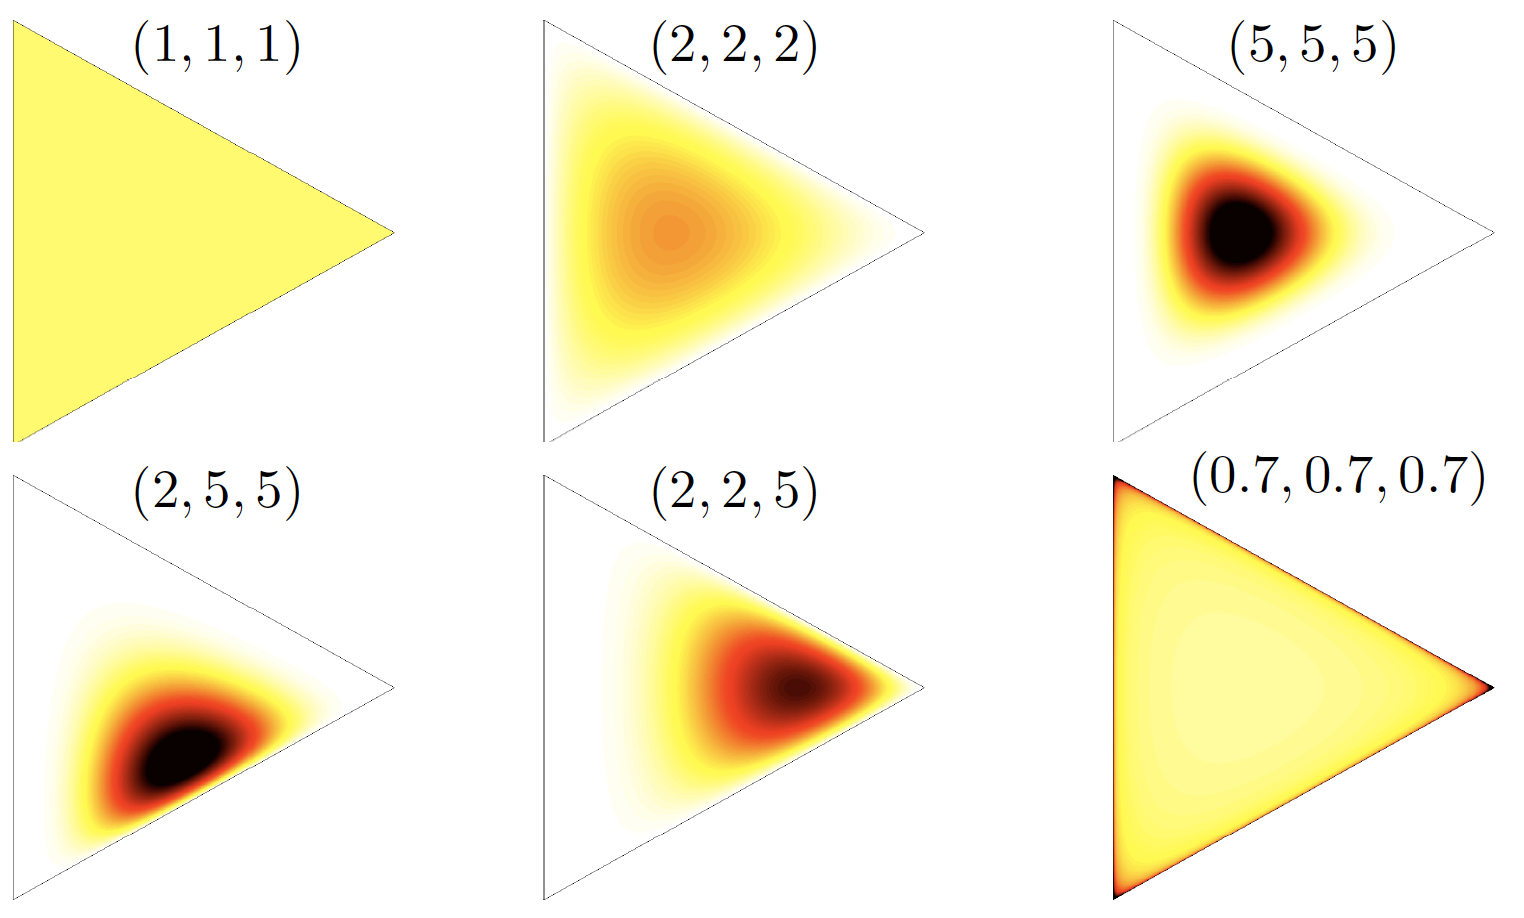
\includegraphics[width = .6\textwidth]{figures_julyan/intro_DP/dirichlet_distribution}
\end{center}
\hfill\textcolor{gray}{[Image by Y.W. Teh]}


The Dirichlet process plays a central role as a Bayesian nonparametric prior \citep{ferguson1973bayesian}.

\begin{definition}{Dirichlet process}
A \alert{Dirichlet process} on the space $\mathcal{Y}$ is a random process $ P $ such that there exist $ \alpha>0 $ (precision parameter) and $ P_0 $ (base/centering distribution)  such that for any finite partition $ \{A_1,\ldots,A_k\} $ of $\mathcal{Y}$, the random vector
$ (P(A_1),\ldots,P(A_k)) $ is Dirichlet distributed
\[ (P(A_1),\ldots,P(A_k))\sim \text{Dir}(\alpha P_0(A_1),\ldots,\alpha P_0(A_k)) \]
\textit{Notation}: $ P \sim \text{DP}(\alpha, P_0) $
\end{definition}
\begin{center}
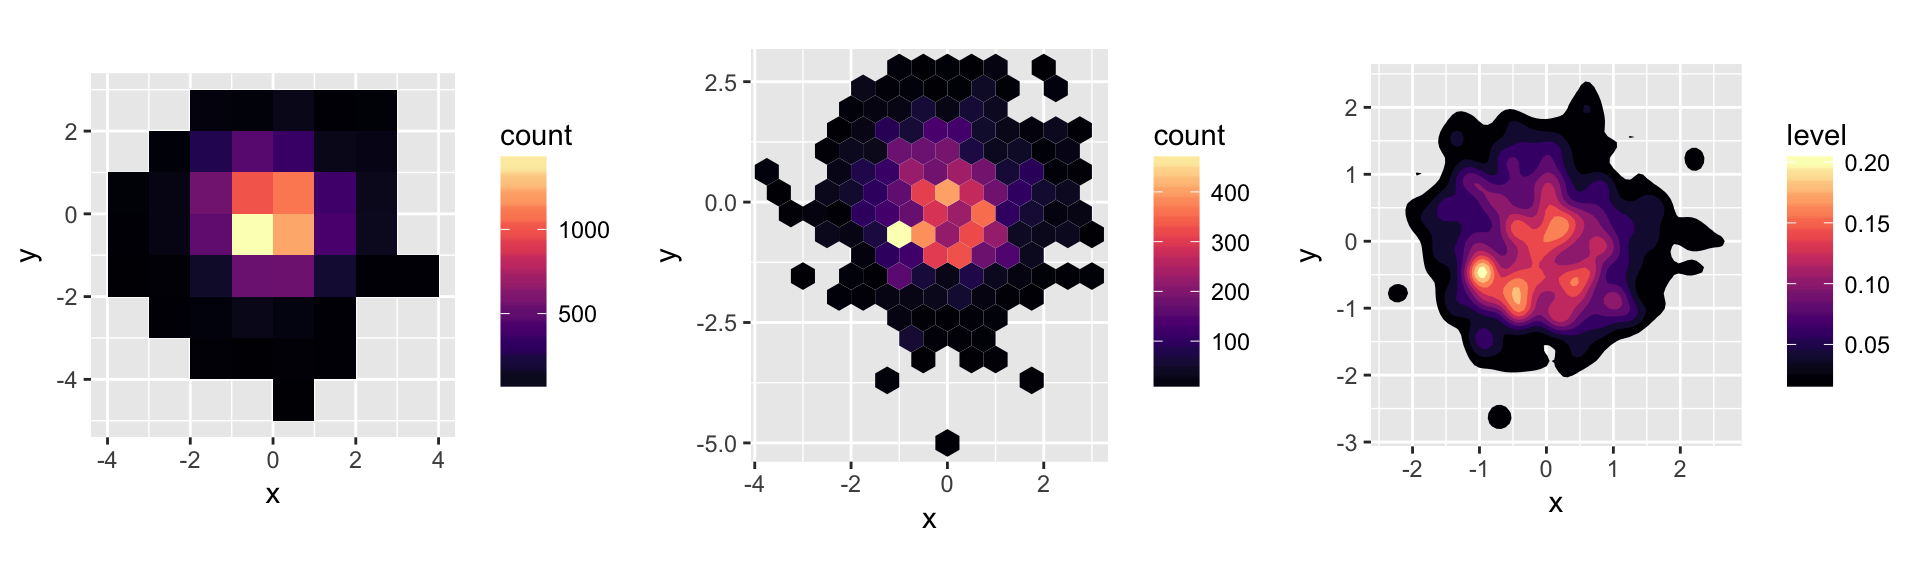
\includegraphics[width=\textwidth]{figures_julyan/intro_DP/DP_marginal}
%\animategraphics[loop, width=\textwidth]{2}{figures_julyan/intro_DP/density_2D_}{1}{10}
\end{center}


%{Moments of Dirichlet process}
\begin{proposition}
Let $P\sim \text{DP}(\PrecisonParam, P_0)$ then for every measurable sets $A, B$ we have
\begin{align*}
    \E[ P(A)] &= P_0(A),\\
    \Var[P(A)] &= \frac{P_0(A)(1-P_0(A))}{1+\PrecisonParam},\\
    \Cov( P(A), P(B) )&=\frac{P_0(A \cap B) - P_0(A)P_0(B) }{1+\PrecisonParam}\label{Dir:Covariance}.
\end{align*}
\end{proposition}


\begin{proof}
We will make use of  $p(A)\sim \Beta(\alpha P_0(A), \alpha (1-P_0(A)))$. From this we obtain 
\begin{equation*}
    \E (p(A)) = \frac{\PrecisonParam P_0(A)}{\PrecisonParam( P_0(A) + 1 - P_0(A) )} = P_0(A)
\end{equation*}
and 
\begin{equation*}
    \Var(p(A))=\frac{\PrecisonParam^2 P_0(A)( 1-P_0(A) )}{\PrecisonParam^2 (\PrecisonParam + 1)}.
\end{equation*}
We derive the covariance term in two cases, firstly taking into consideration the one with $A\cap B = \emptyset$. In that case any space $\Omega$ may be decomposed into three sets: 
$$
\Omega = \{A, B, (A\cup B)^c\}.
$$
Using de Morgan's law the last can be written as $(A\cup B)^c = A^c\cap B^c =: C$. Therefore we may write a joint probability vector
\begin{equation*}
    \big( P(A), P(B), P(A^c\cap B^c) \big)\sim \Dir\big(\PrecisonParam P_0(A), \PrecisonParam P_0(B), \PrecisonParam P_0(C) \big)
\end{equation*}
and hence $\Cov(P(A), P(B)) = -P_0(A)P_0(B)/(1+\PrecisonParam) $. 
In the more general case one may decompose 
\begin{align*}
    A &= (A\cap B) \cup (A\cap B^c)\\
    B &= (B\cap A)\cup (B\cap A^c),
\end{align*}
so that 
\begin{equation*}
    \begin{split}
    \Cov (P(A), P(B)) &= \Cov (P(A\cap B) +P(A\cap B^c), P(B\cap A) + P(B\cap A^c) ) 
    % &=\Cov (P(A\cap B) , P(B\cap A)  ) + \Cov (P(A\cap B),  P(B\cap A^c) ) +\\
    % &+\Cov (P(A\cap B^c), P(B\cap A)  ) + \Cov (P(A\cap B^c),  P(B\cap A^c) ),
    \end{split}
\end{equation*}
and so forth using the linearity of covariance.
\end{proof}



{Marginalizing out the DP}
	Property $\E[ P(A)] = P_0(A)$ can be written equivalently as
\begin{equation*}
    \E( P(A)) = P_0(A) = \int P(A)\ddr \text{DP}(P). 
\end{equation*}

%
%The precision parameter $\PrecisonParam$ in $DP(\PrecisonParam, P_0)$ controls variability of $P(A)$ around $P_0(A)$, so called \textit{base measure} of underlying Dirichlet process. 

A Dirichlet process model can be constructed as a two level sampling model:
\begin{equation*}
    \left \{ \begin{matrix}
P \sim \text{DP}(\PrecisonParam, P_0)\\ 
X|P \sim P,
\end{matrix}\right.
\end{equation*}
i.e. we  sample a probability measure $P$ from the Dirichlet process and then given  $P$, we sample random variables $X_i$.\bigskip

\textcolor{red2}{Marginalizing out $P$}, we obtain the marginal distribution of $X$:
$$X\sim P_0.$$




{Posterior distribution}
	Let $X_{1:n} := (X_1,\ldots, X_n)$ be sampled from the hierarchical model 
\begin{equation*}
    \left \{ \begin{matrix}
P \sim \text{DP}(\PrecisonParam, P_0)\\ 
X_{1:n}|P \simiid P.
\end{matrix}\right.
\end{equation*}
This model is usually used as a building block in a larger hierarchical model, e.g. mixture models, graphs, etc. 
\begin{theorem}[DP posterior distribution] 
The DP is \alert{conjugate}, with posterior equal to
\begin{equation*}
    P|X_{1:n}\sim \text{DP}(\PrecisonParam P_0 + \sum_{i=1}^n\delta_{X_i}).
\end{equation*}
The \alert{predictive distribution}, called \alert{P\'olya urn} or \alert{Blackwell--MacQueen scheme}, is given by
\begin{equation*}
    P(X_{n+1} | X_{1:n}) = \frac{\PrecisonParam}{\PrecisonParam +n} P_0 + \frac{1}{\PrecisonParam + n}\sum_{i=1}^n\delta_{X_i}.
\end{equation*}
\end{theorem}



\begin{proof}
The posterior distribution of $\boldsymbol{a} = (a_1, \ldots, a_k) = ( P(A_1), \ldots, P(A_k) )$ depends on the observations only via their cell counts $\boldsymbol{N}= (N_1, \ldots, N_k)$, $N_j = \# \{ i : X_i \in A_j\}$  (it comes from \textit{tail--free} property), so
\begin{equation*}
  \boldsymbol{a} \vert X_{1:n}\sim \boldsymbol{a} \vert N_{1:k}.
\end{equation*}
The prior  and model are
\begin{equation*}
    \left \{ 
    \begin{matrix}
\boldsymbol{a} \sim \Dir_k (\PrecisonParam P_0(A_1), \ldots, \PrecisonParam P_0(A_k))
\\
\boldsymbol{N}\vert P \sim {\rm Multinom}_k (\boldsymbol{a}).
\end{matrix}\right.
\end{equation*}
This results in the posterior of form 
\begin{align*}
    p(\boldsymbol{a}\vert \boldsymbol{N}) 
    &\propto a_1^{\PrecisonParam P_0(A_1) +N_1-1}\cdots a_k^{\PrecisonParam P_0(A_k)+N_k -1}\\ 
    &= \Dir_k\big( \PrecisonParam P_0(A_1) +N_1, \ldots, \PrecisonParam P_0(A_k) +N_k\big).
\end{align*} \end{proof}
%Property (\ref{Dir:predictive}) is a result of taking the expected value of (\ref{Dir:posterior}). \end{proof}



%----------------
% Combinatorial properties: Number of distinct values
{Combinatorial properties: Number of distinct values}

Assume that the base measure $P_0$ is non-atomic. Then  with probability 1:
$$
X_i\notin\{X_1,\ldots, X_{i-1}\} \Leftrightarrow X_i \sim P_0.
$$
% what means that $X_i$ is a new value.
Let $D_i =  \mathbb{I}(X_i \text{ is a new value})$ and lets denote $K_n=\sum_{i=1}^nD_i$, a number of distinct values $X_1,\ldots, X_n$ with distribution $\mathcal{L}(K_n)$.
\begin{proposition}[Asymptotics for $K_n$]
Random variables $D_i$ are distributed i.i.d. with respect to $Bernoulli(\PrecisonParam/(\PrecisonParam + i - 1))$. Therefore for fixed $\PrecisonParam$ and for $n\rightarrow \infty$ we have:
\begin{enumerate}
    \item[i)] $\E K_n\sim \PrecisonParam \log n \sim \Var(K_n)$
    \item[ii)] $K_n/\log(n)\xrightarrow{a.s.} \PrecisonParam$
    \item[iii)] $(K_n - \E K_n)/\text{sd}(K_n)\rightarrow N(0,1) $
    \item[iv)] $\text{d}_{\text{TV}}\big( \mathcal{L}(K_n), \text{Poisson}(\E K_n) \big)=o \big(1 / \log(n)\big)$ where $$
    \text{d}_{\text{TV}}(P,Q)=\text{sup}|P(A)-Q(A)|
    $$
    over measurable  partition $A$
\end{enumerate}
\end{proposition}



\begin{proof}
\begin{enumerate}
    \item[i)] $\E K_n = \sum_{i=1}^n \frac{\PrecisonParam}{\PrecisonParam+i-1} $ and $ \Var(K_n) = \sum_{i=1}^n\frac{\PrecisonParam(i-1)}{(\PrecisonParam + i -1)^2}$.
    \item[ii)] Since $D_i$'s are $\mathbb{I}$ one may use Kolmogorov law of strong numbers and 
    $$
    \sum_{i=1}^\infty \frac{\Var (D_i)}{ (\log i)^2 }= \sum_{i=1}^\infty \frac{\PrecisonParam(i-1)}{(\PrecisonParam +i-1)^2 (\log i)^2}<\infty$$
    by e.g. the fact that $\sum_i (1/i(\log i)^2)$ converges.
    \item[iii)]By Lindeberg central limit theorem.
    \item[iv)] This is implied from Chein--Stein approximation. %https://faculty.math.illinois.edu/~psdey/414CourseNotes.pdf 
\end{enumerate}
\end{proof}


A central limit theorem for independent random variables (possibly not identically distributed).

\begin{theorem}[Lindeberg central limit theorem]
Suppose $X_i$ are i.i.d. such that $\E X_i = \mu_i$ and $\Var X_i = \sigma_i^2 <\infty$. Define $Y_i = X_i - \mu_i,\ T_n = \sum_{i=1}^n Y_i,\ s_n^2 = \Var (T_n) = \sum_{i=1}^n\sigma_i^2$. Then provided that
\begin{equation*}
    \forall \epsilon > 0\quad \frac{1}{s_n^2}\sum_{i=1}^n\E \big(Y_i^2 \mathbb{I}(|Y_i|>\epsilon s_n) \big)\xrightarrow{n\rightarrow \infty} 0 \text{[Lindeberg condition],}
\end{equation*}
we have the central limit theorem: $T_n/s_n \xrightarrow{\small{d}}N(0,1)$.
\end{theorem}





%------------
% Combinatorial properties: Distribution of distinct values
{Combinatorial properties: Distribution of distinct values}
	We have now the limits of $K_n$ and we know its approximate distribution $\mathcal{L}(K_n)$. The \alert{exact distribution of $K_n$} is:
\begin{proposition}[Distribution of $K_n$]
If $P_0$ is non-atomic then 
\begin{equation}\label{distr_of_Kn}
    P(K_n=k) = \mathfrak{C}_n(k) n!\PrecisonParam ^k \frac{\Gamma(\PrecisonParam)}{\Gamma(\PrecisonParam+n)},
\end{equation}
where 
\begin{equation}\label{mathfrakC_def}
\mathfrak{C}_n(k)=\frac{1}{n!}\sum_{S\in\mathfrak{J}_n(k)} \prod_{j\in S}j    
\end{equation}
and $\mathfrak{J}_n(k)=\{ S\subset \{ 1,\ldots,n-1\},\ |S|=n-k \}$.
\end{proposition}

 Recall the definition of the \alert{Gamma function} $\Gamma(x)=\int_0^\infty u^{x-1}e^{-u}du$.
 




Let us consider when we may deal with events $K_n = k$: we have two cases
\begin{equation*}
    \left \{ \begin{matrix}
K_{n-1}=k-1 \text{ and } X_n \text{ is a new value}\\
K_{n-1} = k \text{ and } X_n \text{ is not a new value}.
\end{matrix}\right.
\end{equation*}
 This results in
% either in proceeding case $K_{n-1}$ we have $K_{n-1}=k-1 $ and $X_n$ is a new value or we have $K_{n-1} = k$ and $X_n$ does not take new value.
\begin{equation}\label{CombinatorialProperties}
    p_n(k,\PrecisonParam) := P(k_n = k|\PrecisonParam) = \frac{\PrecisonParam}{\PrecisonParam +n -1 }p_{n-1} (k-1,\PrecisonParam)+\frac{n-1}{\PrecisonParam +n -1}p_{n-1}(k,\PrecisonParam).
\end{equation}
Now let us remark that $\mathfrak{C}_n(k)=p_n(k,\PrecisonParam =1)$. Therefore
\begin{equation}\label{mathfrakC_property}
    \mathfrak{C}_n(k)=\frac 1n \mathfrak{C}_{n-1}(k-1)+\frac{n-1}{n}\mathfrak{C}_{n-1}(k).
\end{equation}
By induction over $n$: first we check case $n=1$:
\begin{equation*}
    p_1(1,\PrecisonParam)=\mathfrak{C}_1(1)\frac{\PrecisonParam}{\PrecisonParam}=\mathfrak{C}_1(1).
\end{equation*}
To check case $n>1$ we use (\ref{distr_of_Kn}) and then (\ref{CombinatorialProperties}):
\begin{equation*}
    \begin{split}
        p_n(k,\PrecisonParam)&=\frac{\PrecisonParam}{\PrecisonParam +n -1 }p_{n-1} (k-1,\PrecisonParam)+\frac{n-1}{\PrecisonParam +n -1}p_{n-1}(k,\PrecisonParam) \\
        &=\frac{\PrecisonParam}{\PrecisonParam +n -1 }\mathfrak{C}_{n-1}(k-1)(n-1)!\PrecisonParam^{k-1}\frac{\Gamma (\PrecisonParam)}{\Gamma(\PrecisonParam+n-1)} +\\
        &+\frac{n-1}{\PrecisonParam +n -1}\mathfrak{C}_{n-1}(k)(n-1)!\PrecisonParam^{k}\frac{\Gamma (\PrecisonParam)}{\Gamma(\PrecisonParam+n-1)}\\
        &=\frac{\PrecisonParam^k}{\PrecisonParam+n-1}(n-1)!\frac{\Gamma(\PrecisonParam)}{ \Gamma(\PrecisonParam+n-1) }n\bigg(\frac 1n \mathfrak{C}_{n-1}(k-1) + \frac{n-1}{n} \mathfrak{C}_{n-1}(k)\bigg)\\
        &=\mathfrak{C}_{n}(k)n!\PrecisonParam^k\frac{\Gamma(\PrecisonParam)}{\Gamma(\PrecisonParam+n)},
    \end{split}
\end{equation*}
which proves property (\ref{distr_of_Kn}).

To prove (\ref{mathfrakC_def}) let use define a polynomial $A_n(s)$ as $A_n(s) = \sum_{i=1}^\infty \mathfrak{C}_n(k)s^k$. Then using (\ref{mathfrakC_property}) polynomial $A_n(s)$ can be written as
\begin{equation*}
\begin{split}
    A_n(s)&=\sum_{k=1}^\infty \bigg(  \frac 1n \mathfrak{C}_{n-1}(k-1)+\frac{n-1}{n}\mathfrak{C}_{n-1}(k)   \bigg) s_k\\
    &=\frac{1}{n}( s A_{n-1}(s) +(n-1) A_{n-1}(s) )=\frac{s+n-1}{n}A_{n-1}(s)\\
    &=\ldots=A_1(s)\prod_{j=2}^n\frac{s+j-1}{j}=\frac{s(s+1)\cdot\ldots\cdot(s+n-1)}{n!}.
\end{split}
\end{equation*}
Last equality implies from the fact that $\mathfrak{C}_1(k)=\ind\{k=1\}$ and hence $A_1(s)=s$. Checking terms after the expansion finishes the proof of (\ref{mathfrakC_def}).







%------------
% Combinatorial properties: CRP
{Combinatorial properties: Chinese Restaurant process}
A culinary metaphor of the \alert{random partition} induced by the DP. Customers join tables with probability proportional to \alert{$n_j$}, the number of clients already sitting, or sit at new table with probability  proportional to \alert{$\PrecisonParam$}.
\begin{center}
	\includegraphics[width = .5\textwidth]{figures_julyan/intro_DP/CRP}
\end{center}

\begin{proposition}[Chinese Restaurant process]
A random sample $X_{1:n}$ from a DP with precision parameter $\PrecisonParam$ induces a partition of $\{1,\ldots,n\}$ into $k$ sets of sizes $n_1,\ldots,n_k$ with probability 
\begin{equation*}
    p(n_1,\ldots,n_k)=p(\{n_1,\ldots,n_k\})=\PrecisonParam^k\frac{\Gamma(\PrecisonParam)}{\Gamma(\PrecisonParam+n)}\prod_{j=1}^k\Gamma (n_j).
\end{equation*}
\end{proposition}


\begin{proof}
	We use the P\'olya urn scheme slightly changed by using $n_1,\ldots, n_k$
\begin{equation*}
    P(X_{n+1}|X_{1:n})=\frac{\PrecisonParam}{\PrecisonParam + n}P_0 + \frac{1}{\PrecisonParam + n}\sum_{j=1}^kn_j\delta_{X^*_j}.
\end{equation*}
    By exchangeability, the distribution of $\{n_1,\ldots, n_k\}$ does not depend on the order of the observations. Let's compute $p(n_1,\ldots, p_k)$ as the probability of one draw where the first table consists of first $n_1$ observations etc. 
    
    To proceed, let us use P\'olya urn scheme: we denote $\bar{n}_j=\sum_{i=1}^jn_i$ and hence $\bar{n}_k=n$, the total number of observations. We can observe the following pattern: first ball open new table, following $n_j-1$ ones fill in that table and so forth. That quantity can be rewritten as 
    $$
    \frac{\PrecisonParam^k}{\PrecisonParam(\PrecisonParam+1)\ldots(\PrecisonParam+n-1)}\prod_{j=1}^k(n_j-1)!,
    $$
where one can rewrite both terms using Gamma function $\Gamma(x)=\int_0^\infty u^{x-1}e^{-u}du$: the first  term  can be written as 
$$
\frac{\PrecisonParam^k}{\PrecisonParam(\PrecisonParam+1)\ldots(\PrecisonParam+n-1)}=\frac{\Gamma(\PrecisonParam+n)}{\Gamma(\PrecisonParam)},
$$
while the second one as
$(n_j-1)!=\Gamma(n_j)$.

One should remark that for ordered partitions we have 
$$
\bar{p}(n_1,\ldots,n_k)=\frac{p(n_1,\ldots,n_k)}{k!}.
$$
\end{proof}



%
%%------------
%% Combinatorial properties: Ewens
%{Combinatorial properties: Ewens sampling formula}
%
%
%



%------------
% Combinatorial properties: Ewens
{Combinatorial properties: Ewens sampling formula}

Ewens sampling formula (ESF), presented originally by \citet{ewens1972sampling}, is the distribution of multiplicities $m=(m_1,\ldots, m_n)$, $m_\ell$ is the number of groups of size $\ell$.
Also known as allelic partitions in population genetics, when there is no selective difference between types: null hypothesis in non Darwinian theory.
See also \citet{antoniak1974mixtures}.

\begin{proposition}[Ewens sampling formula]\label{ESF}
The distribution of the multiplicities $(m_1,\ldots, m_n)$ induced by a DP is
\begin{equation*}
    p(m_1,\ldots, m_n)=\frac{\PrecisonParam^k}{\PrecisonParam_{(n)}}\frac{n!}{\prod_{\ell=1}^n \ell^{m_\ell}m_\ell!}.
\end{equation*}
\end{proposition}\bigskip

Notation $n_{(k)}:=n(n-1)\cdots(n-k+1)$.



%\vskip -1cm
%\begin{center}
%	\includegraphics[width = .6\textwidth]{figures_julyan/CRP}
%\end{center}


\begin{proof}
Two steps: 1) Compute probability of particular sequence of $X_1, \ldots, X_n$ in given class $(m_1,\ldots,m_n)$, note that all such sequences are equally likely and 2) multiply obtained quantity by the number of such sequences. 

\begin{itemize}
    \item[1)] Consider a sequence $X_1,\ldots, X_n$ such that $X_1, \ldots, X_{m_1}$ occur each only once, then the next $m_2$ occur only twice and so on. This sequence has probability which may be obtained by the P\'olya Urn scheme in the same fashion as CRP:
    \begin{equation*}
        \frac{\PrecisonParam^{m_1} (\PrecisonParam \cdot 1)^{m_2} \ldots \big( \PrecisonParam \cdot 1 \cdot\ldots \cdot (n-1) \big)^{m_n}  }{\PrecisonParam_{(n)}}=\frac{\PrecisonParam^k}{\PrecisonParam_{(n)}}\prod_{\ell=1}^n ((\ell-1)!)^{m_\ell}.
    \end{equation*}
%    Each term in the numerator comes from $m_\ell$ species observed $\ell$ times.
    \item[2)] Number of sequences $X_1,\ldots,X_n$ with frequencies $(m_1, \ldots, m_n)$ is a number of ways of putting $n$ distinct objects into bins, so called multinomial coefficient. Since ordering of the $m_\ell$ bins of frequency $\ell$ is irrelevant,  divide by $m_\ell!$:
    \begin{equation*}
        \frac{1}{\prod_{l=1}^n (m_\ell)!}
        \begin{pmatrix}
n\\ 
1\times \# m_1, 2\times \# m_2, \ldots, n\times \# m_n
\end{pmatrix}
= \frac{n!}{\prod_{\ell=1}^n m_\ell!(\ell!)^{m_\ell}}
    \end{equation*}
\end{itemize}
To finish one needs to multiply results obtained in 1) and 2). \end{proof}





%-------------
% Stick-breaking

{Stick-breaking representation}
The \alert{DP} has almost surely \alert{discrete} realizations (Sethuraman, 1994)

\begin{minipage}{.55\textwidth}
$$P=\sum_{j=1}^{\infty}\pi_{j}\delta_{\theta_{j}}\,\text{ }$$
\begin{itemize}
\item locations $\theta_{j}\simiid G_{0}$ %(Sethuraman 1994)%\citp{se}
\item %weights $p_{j}$ defined by 
weights $\pi_{j}=\tilde \pi_j\prod_{l<j}(1-\tilde \pi_{l})$ with $\tilde \pi_{j}\simiid Beta(1,\alpha)$,
\end{itemize}\medskip
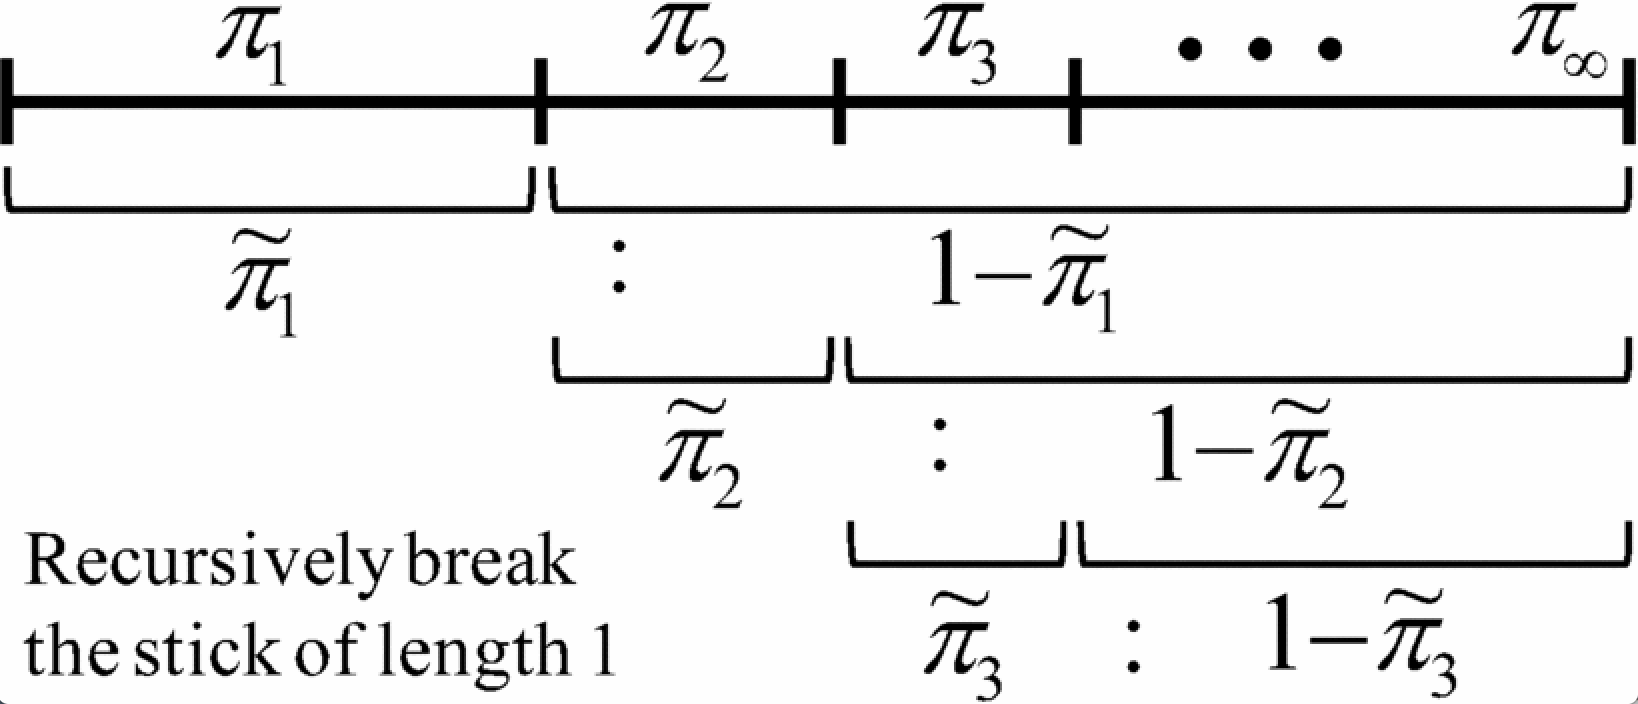
\includegraphics[width=\textwidth]{figures_julyan/intro_DP/sb}
\end{minipage}\hskip.5cm
\begin{minipage}{.4\textwidth}
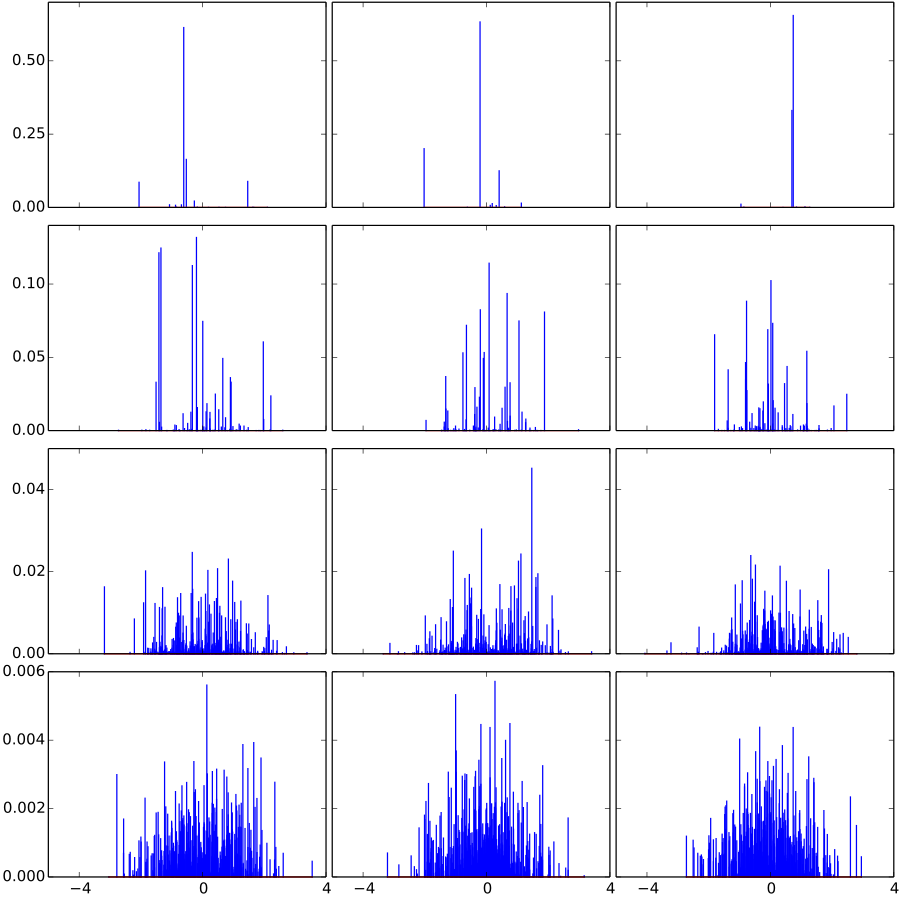
\includegraphics[width=\textwidth]{figures_julyan/intro_DP/DP}
\end{minipage}



{Stick-breaking representation}

A constructive representation of the DP due to \citet{sethuraman1994constructive}.
\begin{theorem}[Stick-breaking]\label{theorem:sethuraman}
If $V_1, V_2, \ldots \simiid Be(1, \PrecisonParam)$ and $\phi_1, \phi_2, \ldots \simiid P_0$ are i.i.d. variables, then define $p_1=V_1$ and 

$$
p_j=V_j \prod_{1\leq l \leq j}(1-V_l)
$$ 
then 
$$
P=\sum_{i=1}^\infty p_i\delta_{\phi_i}\sim \text{DP}(\PrecisonParam, P_0).
$$
\end{theorem}



\begin{lemma}
For independent $\phi\sim P_0$ and $V\sim Be(1,\PrecisonParam)$ the DP is the only solution of the distributional equation 
\begin{equation*}\label{Dir:distributional_equation}
    P \sim V\delta_\phi + (1-V)P, 
\end{equation*}
where $P\sim \text{DP}(\PrecisonParam, P_0)$.
\end{lemma}

%We say that such a RPM is solution of (\ref{Dir:distributional_equation}) if $P$ is independent of $(V, \phi)$ and if for every measurable partition $(A_1, \ldots, A_k)$ of $X$ both sides of (\ref{Dir:distributional_equation}) are random vectors equal in distribution in $\mathbb{R}^k$. 
%Proof of the lemma follows from properties of Dirichlet distribution. We are ready now to prove the  theorem.



\begin{proof}
1) The weights $(p_1, p_2,\ldots)$ need to form a probability vector. The leftover mass at stage $j$ is 
$$
1-\bigg(\sum_{i=1}^j p_i\bigg)=\prod_{i=1}^j(1-V_i) =: R_j.
$$
One may notice that $R_j$ is decreasing and for every $j$ we have $R_j\in [0,1]$, hence we obtain almost sure convergence which is equivalent with convergence in mean. Therefore
$$
\E R_j=\E \prod_j (1-V_j)= \prod_j \E(1-V_j) = \bigg( \frac{\PrecisonParam}{\PrecisonParam + 1}\bigg)^j \rightarrow 0.
$$
So ($p_1, \ldots$) is a probability vector almost surely and $P$ is a probability measure almost surely. 



2) Now one may write 
$$
P=p_1\delta_{\phi_1}+\sum_{j=2}^\infty p_j\delta_{\phi_j} = V_1\delta_{\phi_1}+(1-V_1)\sum_{j=1}^\infty \Tilde{p_j}\delta_{\Tilde{\phi}_j},
$$
where $\Tilde{p}_j=\frac{p_{j+1} }{1-V_1}=V_{j+1}\prod_{l=2}^j(1-V_l)$ and $\Tilde{\phi}_j=\phi_{j+1}$, then $(\Tilde{p}_j)$ and $(\Tilde{\phi}_j)$ satisfy the same distributional definitions as $(p_j)$ and $(\phi_j)$, hence $\Tilde{P}\sim P$ and so $P$ is solution of the Lemma equation (\ref{Dir:distributional_equation}) whose only solution is the DP.
\end{proof}







%------------
% Normalization
{DP as a normalized Gamma process}
The DP can be obtained by \alert{normalizing a Gamma process}. It is a generic way to obtain random probability measures from almost surely finite random measures. Let us restrict to $\mathcal{Y}=\mathbb{R}$.
\begin{definition}
Gamma process on $\mathbb{R}_+$ is a process $(S(u):u \geq 0)$ with independent increments satisfying
\begin{equation*}
    \forall u_1: 0 \leq u_1 \leq u_2:\quad S(u_2) - S(u_1)\simind Ga(u_2-u_1,1).
\end{equation*}
This ensures that the process has non-decreasing right continuous sample path $u\mapsto S(u)$.
\end{definition}

\begin{theorem}
For every $\PrecisonParam>0$ and for every cumulative distribution function $G$, a random cumulative distribution function such that
\begin{equation*}
    F(t) = \frac{S(\PrecisonParam G(t))}{S(\PrecisonParam)}
\end{equation*}
is the distribution of a $\mathsf{DP}(\PrecisonParam,G)$.
\end{theorem}

\begin{proof}
For any set of $t_i$ satisfying $-\infty = t_0 < t_1 < \ldots < t_k = \infty$ we have 
$$
S(\PrecisonParam G(t_i)) - S(\PrecisonParam G(t_{i-1})) \sim Ga\big( \PrecisonParam G(t_i)-\PrecisonParam G(t_{i-1}),1\big).
$$
Use property that if $Y_i \simind Ga(\PrecisonParam_i, 1)$ then $(Y_1, \ldots, Y_n)/\sum_i Y_i \sim \Dir_n (\PrecisonParam_1,\ldots, \PrecisonParam_n)$ to obtain 
$$
\big(F(t_1)-F(t_0), \ldots, F(t_k) - F(t_{k-1}) \big) \sim \Dir_k\big(\PrecisonParam G(t_1) -\PrecisonParam G(t_0), \ldots, \PrecisonParam G(t_k) -\PrecisonParam G(t_{k-1})\big).
$$
Hence the definition of DP holds for every partition in intervals. These form a measure determining class, so that the definition holds for every partition in general. 
\end{proof}








%------------
% P\'olya Urn charact
{Definition via the P\'olya urn scheme}
A P\'olya sequence with parameter $\PrecisonParam P_0$ is a sequence of random variables $X_1, \ldots, X_n$ whose joint distribution satisfies
\begin{equation*}
    X_1 \sim P_0,\ X_{n+1}|X_1,\ldots,X_n\sim \frac{\PrecisonParam}{\PrecisonParam + n}P_0 + \frac{1}{\PrecisonParam + n}\sum_{i=1}^n \delta_{X_i}.
\end{equation*}

\begin{theorem}
If $X_1,X_2,\ldots $ is a P\'olya sequence then exists random probability measure $P$ such that $X_i|P\simiid P$ and $P\sim \text{DP}(\PrecisonParam, P_0)$.
\end{theorem}

\begin{proof}
We can consider P\'olya sequence as an outcome of P\'olya urn, we see that it is exchangeable. By de Finetti theorem exists such probability measure $P$ such that $X_i|P \simiid P$. So far we have proved existence of the DP and know that DP generates a P\'olya sequence. Since the RPM given by de Finetti's theorem is unique this proves that
$P\sim \text{DP}(\PrecisonParam, P_0)$.
\end{proof}



%%%%%%%%%%%%%%%%%%%%%%%%%%%%%%%%%%%%%%%%%%%%%%%%%%%%%%%%%%%%%%%%%%%%%%%%%%%%%%
\section{Mixtures and model-based clustering}
%%%%%%%%%%%%%%%%%%%%%%%%%%%%%%%%%%%%%%%%%%%%%%%%%%%%%%%%%%%%%%%%%%%%%%%%%%%%%%



{A {parametric} approach}
 Mixture model with $K$ components
	
	$$G = \sum_{k=1}^K \pi_k \delta_{\phi_k}$$
	
	$\delta_{\phi_k}$ is a point mass at ${\phi_k}$.
	
	$G$ is to be understood as a $K$-faceted dice. The  mixture density is:
	$$p(X|\pi,\phi) = \sum_{k=1}^K \pi_k p(x|\phi_k)$$
	
\begin{center}
		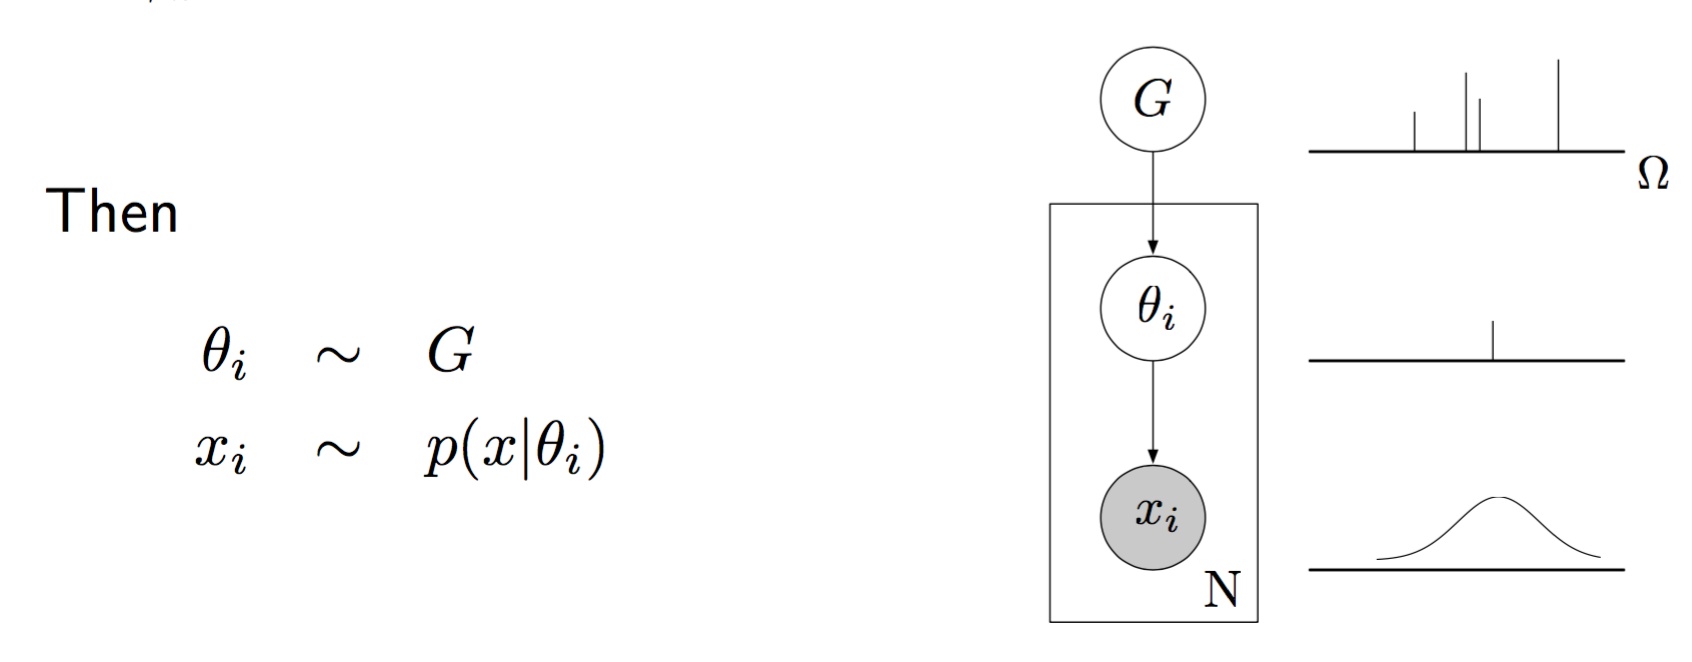
\includegraphics[width=.8\textwidth]{figures_julyan/mixtures/plate_mixture}
\end{center}




{A {Bayesian parametric} approach}
	 \alert{Bayesian}   mixture models with $K$ components
	
We need a distribution over the probability measure (aka dice) $G$, that is a distribution over weights or classes $\pi = (\pi_1,\ldots,\pi_K)$ and over mean and covariance (for 2-dimensional data) $\phi_k = (\mu_k,\Sigma_k)$

\begin{itemize}
	\item $\pi\sim \text{Dirichlet}(\alpha/K, \ldots,\alpha/K)$
	\item $(\mu_k,\Sigma_k)\sim \text{Normal}\times\text{Inverse-Wishart}$
\end{itemize}
This makes $G = \sum_{k=1}^K \pi_k \delta_{\phi_k}$ a random dice

\begin{center}
		\includegraphics[width=.8\textwidth]{figures_julyan/mixtures/plate_bayes_mixture}
\end{center}


{Choosing $K$}
There are several options for choosing $K$
\begin{itemize}
	\item Model selection with information criteria: AIC, BIC, or cross-validation, etc
	\item Hierarchical model, with a prior on $K$
	\item Be nonparametric, and let $K$ get large... possibly infinite.
\end{itemize}
	




{A {Bayesian nonparametric} approach}
	 \alert{Bayesian nonparametric}   mixture models
	 
	 We now move to $G$ being an infinite sum $G = \sum_{k=1}^\infty \pi_k \delta_{\phi_k}$.
	
We need a distribution over this infinite dice $G$, that is exactly what the \alert{Dirichlet process} does. It is parameterized by the precision parameter $\alpha$ and the base measure $G_0$.


\begin{itemize}
	\item $\pi = (\pi_1,\pi_2,\ldots)\sim \text{GEM}(\alpha)$
	\item $\phi_k\sim G_0$
\end{itemize}

\begin{center}
		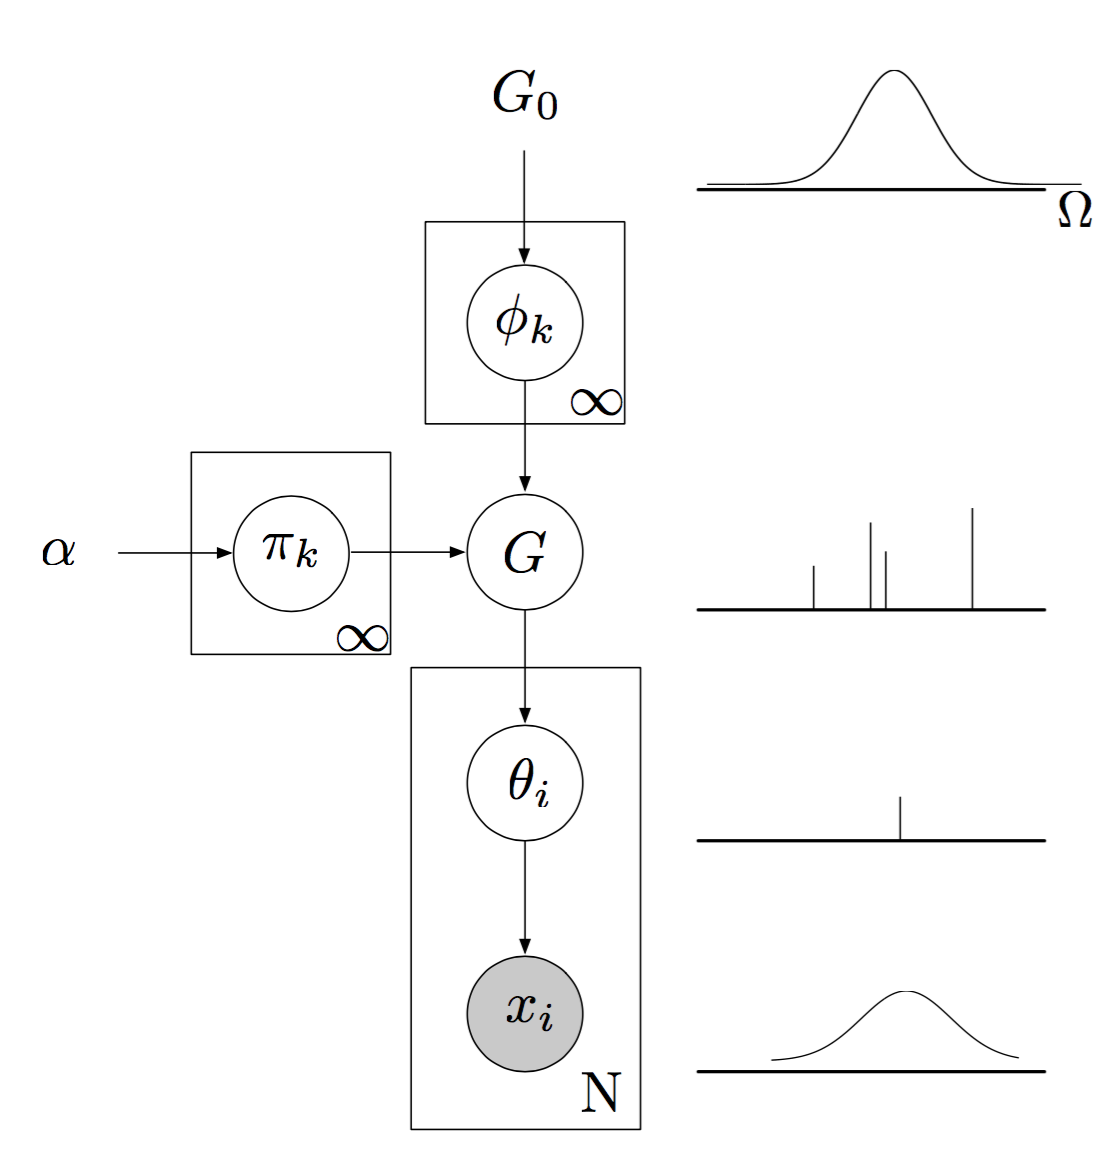
\includegraphics[height=.4\textheight]{figures_julyan/mixtures/plate_SB_mixture}
\end{center}




{Posterior sampling}
Markov chain Monte Carlo (MCMC) methods:
\begin{itemize}
\item \alert{Marginal methods}: marginalizing over the posterior DP $P$, and sampling using the posterior P\'olya urn scheme \citep[easy in conjugate case, see][]{neal2000markov}
\item \alert{Conditional methods}: sampling a finite but sufficient number of parameters
 \citep{ishwaran2001gibbs}. \alert{BNPdensity} R package \citep{arbel2021BNPdensity}.
\end{itemize}
Variational approximations \citep{blei2006variational}




{Warning on interpretation of $K_n$}

	Consider a simple DP mixture model with
	\begin{itemize}
		\item  Gaussian base measure, 
		\item Gaussian kernel,
		\item where data are sampled  iid from some distribution.
	\end{itemize}
	
Then the \alert{posterior on $K_n$ is inconsistent} \citep{miller2013simple}.

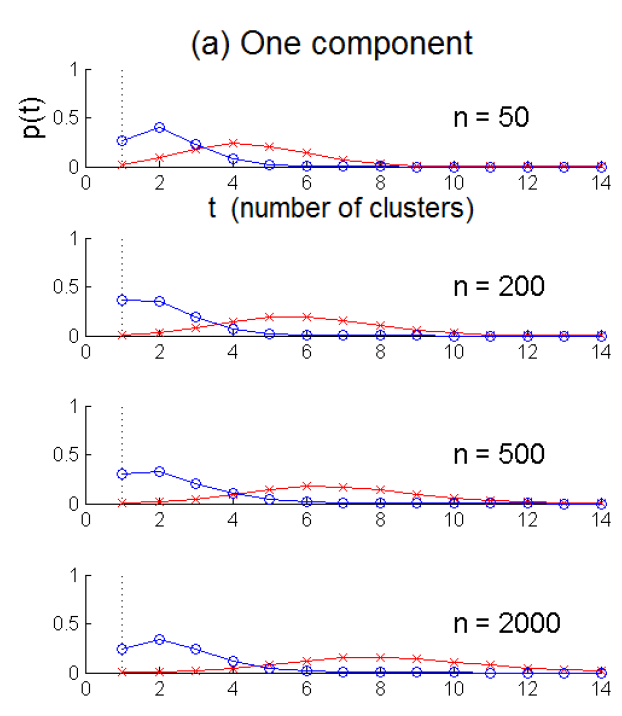
\includegraphics[width=\textwidth]{figures_julyan/mixtures/miller_DP}


From \citet{miller2013simple} (here $K_n$ is denoted $T_n$):\bigskip

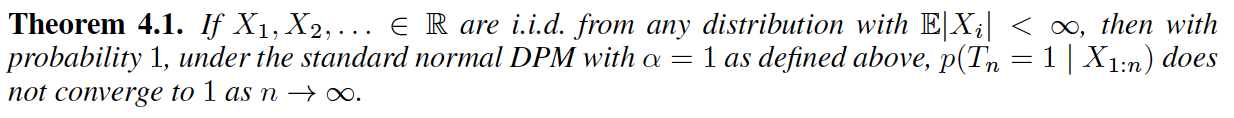
\includegraphics[width=\textwidth]{figures_julyan/mixtures/miller_inconsistency1}\bigskip

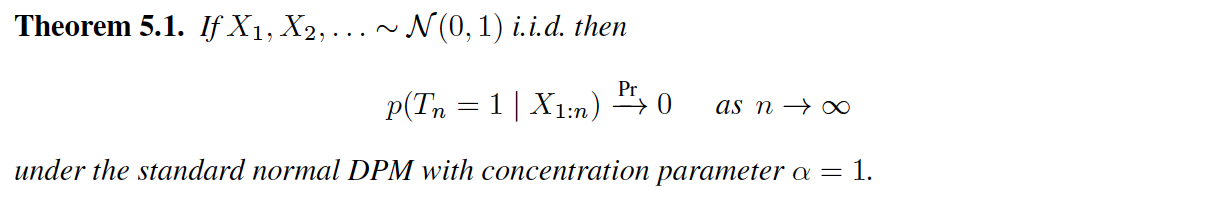
\includegraphics[width=\textwidth]{figures_julyan/mixtures/miller_inconsistency2}\bigskip


But there is some hope...




{Bayesian decision theory}
	From decision theory: a Bayes estimator minimizes a posterior expected loss.
	
\begin{equation*}
\hat{a}_L = \arg \inf_{a \in A} \mathbb{E}_{\pi(\theta)}[L_a(\theta)].
\end{equation*}

Examples with Euclidean parameter spaces:
\begin{itemize}
	\item $L^2$, squared loss $\longrightarrow$ posterior mean
	\item $L^1$, absolute loss $\longrightarrow$ posterior median
	\item $0-1$ loss  $\longrightarrow$ mode a posteriori (MAP)
\end{itemize}


{Deriving an optimal clustering}

The posterior expected loss of clustering $c'$, denoted by $L(c')$, is obtained by \alert{averaging the loss with respect to posterior weight}
$$L(c') = \sum_{c\in\Ac_n} L(c,c')p(c|\bx),$$
and the decision is taken by choosing the best

\begin{equation*}
\hat c = \arg \min_{c' \in \Ac_n} \sum_{c\in\Ac_n} L(c,c')p(c|\bx)
\end{equation*}
Several losses have been considered:
	\begin{itemize}
		\item 0-1 loss \citep{rajkowski2019analysis},
		\item Binder loss \citep{dahl2006model},
		\item Variation of information \citep{wade2018bayesian}.
	\end{itemize}


{Simplest loss: $L_{0-1}$}

\begin{align*}
	L_{0-1}(c') = \sum_{c\in\Ac_n} L_{0-1}(c,c')p(c|\bx) &= \sum_{c\in\Ac_n,\,c\neq c'} p(c|\bx),\\
	& = 1 - p(c'|\bx)
\end{align*}
which is to say that the expected loss of $c'$ is \alert{all the posterior mass except that of $c'$.} So that it is easily minimized at the value $c'$ which has \alert{maximum} posterior weight:
$$\hat c =  \arg \min_{c' \in \Ac_n} L_{0-1}(c') =   \arg \max_{c' \in \Ac_n} p(c'|\bx):= MAP.$$

Negative results by \citet{rajkowski2019analysis} show that the \alert{mode a posteriori (MAP) is inconsistent}.
	


{Variation of information}
\alert{Variation of information} (VI) by \citet{meila2007comparing} for cluster comparison. From information theory, compares information in two clusterings with information shared between the two clusterings:
\begin{align*}
&\VI(\bc,\widehat{\bc})=\En(\bc)+\En(\widehat{\bc})-2\I(\bc,\widehat{\bc})
\end{align*}



{Variation of information}
\citet{wade2018bayesian} 
compare Binder and VI:\bigskip

\begin{center}
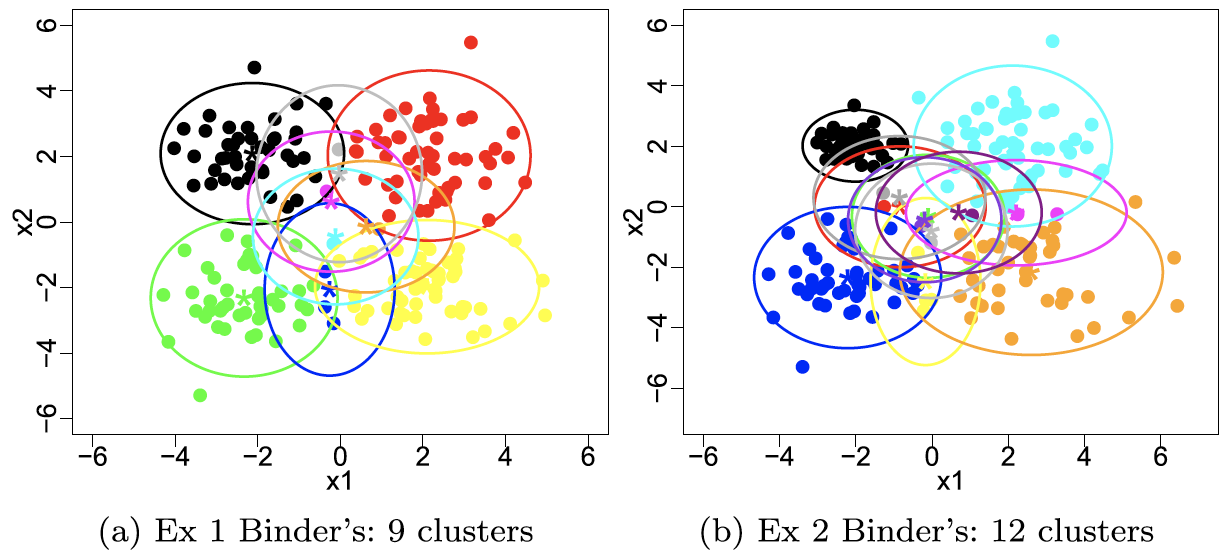
\includegraphics[width=.7\textwidth]{figures_julyan/mixtures/wade_example_binder}
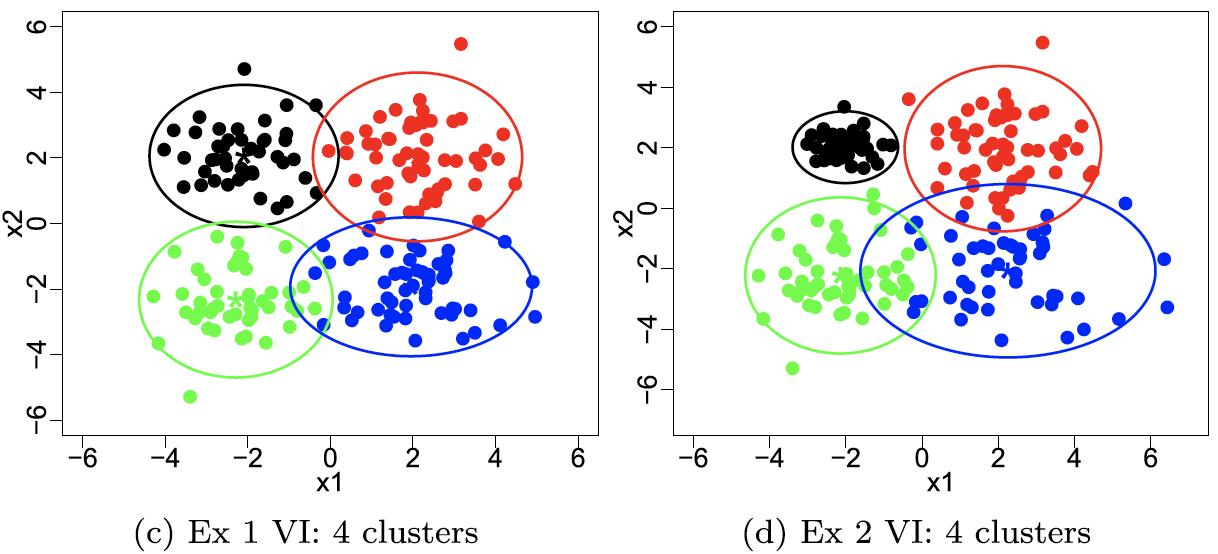
\includegraphics[width=.7\textwidth]{figures_julyan/mixtures/wade_example_VI}	
\end{center}



{Variation of information}
\citet{wade2018bayesian} 
also provide \alert{credible balls} around the estimated clustering, based on Hasse diagram:\bigskip

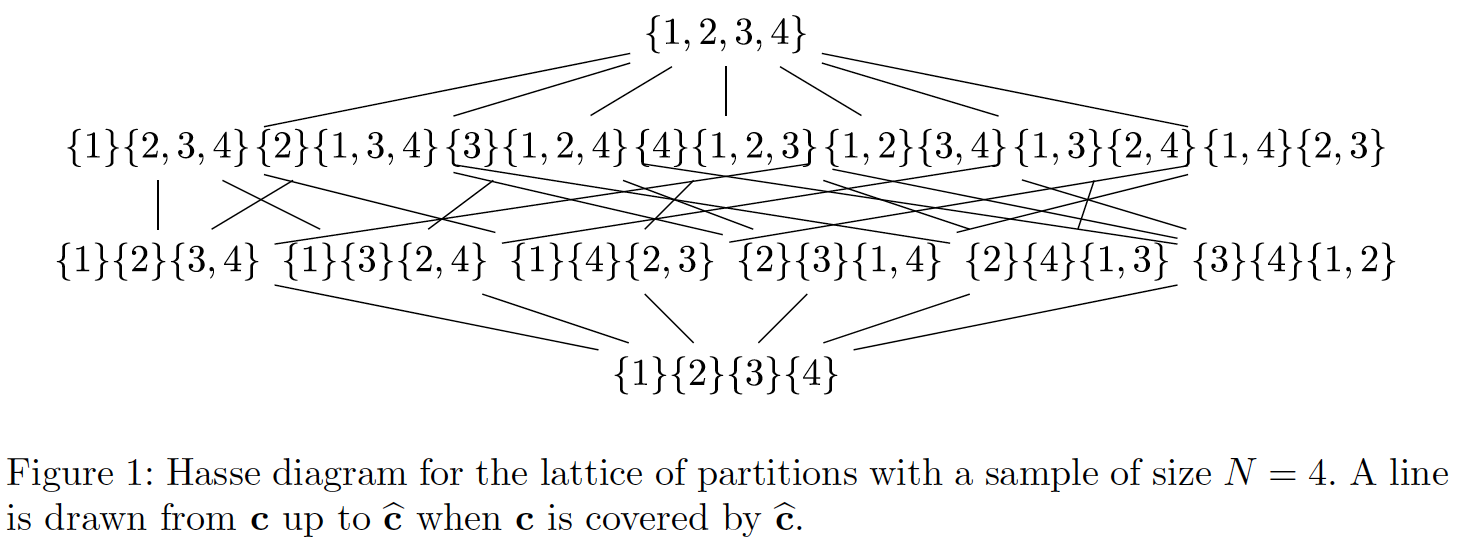
\includegraphics[width=\textwidth]{figures_julyan/mixtures/hasse_diagram}



%%%%%%%%%%%%%%%%%%%%%%%%%%%%%%%%%%%%%%%%%%%%%%%%%%%%%%%%%%%%%%%%%%%%%%%%%%%%%%
\section{Priors beyond the Dirichlet process}
%%%%%%%%%%%%%%%%%%%%%%%%%%%%%%%%%%%%%%%%%%%%%%%%%%%%%%%%%%%%%%%%%%%%%%%%%%%%%%





 
 {Need for a power-law for $K_n$}
 
 	\citet{newman2005power,clauset2009power} show that ``\textit{Power-law distributions occur in many situations of scientific interest and have
significant consequences for our understanding of natural and man-made phenomena}''.
		\begin{center}
			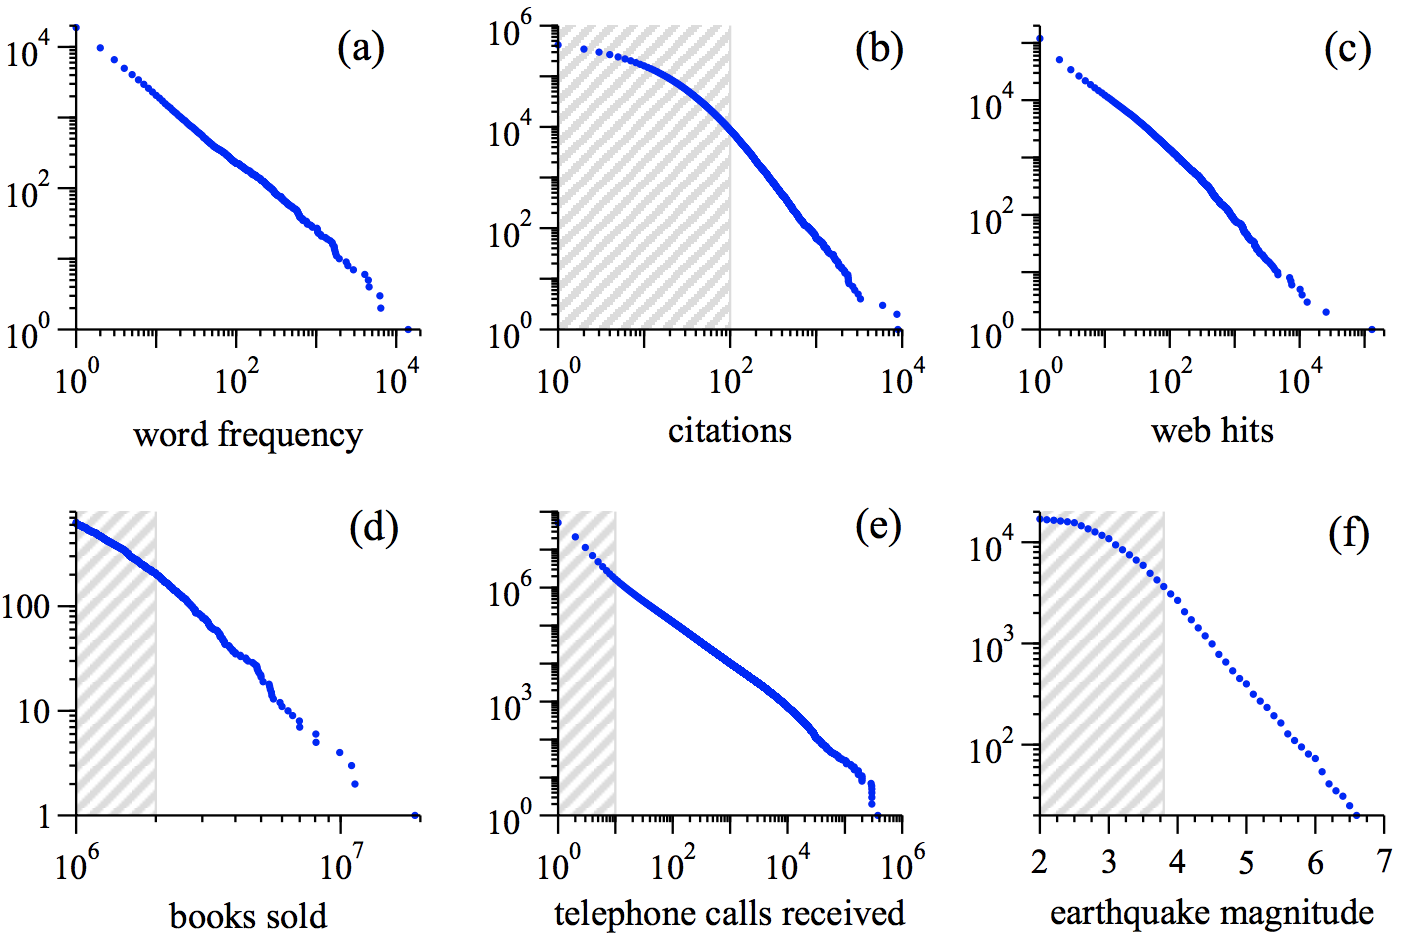
\includegraphics[width=.7\textwidth]{figures_julyan/beyond_DP/power_laws_newman}
		\end{center}
		\hfill\textcolor{gray}{[Image from \citet{newman2005power}]}

		Hence the need to depart from $K_n\sim \alpha \log n$ induced by a Dirichlet process.
 

 
\subsubsection{Chinese restaurant process}

Consider discrete data $X_1,\ldots X_n\vert P\simiid P$, and $ P \sim \mathcal{Q}$

Features $k_n\leq n$ unique values $X_1^*,\ldots,X_{k_n}^*$ with resp. frequencies $n_1,\ldots,n_{k_n}$\medskip 


{Discrete random probability measures} are characterized by  \alert{predictive distr.}
\medskip

\alert{Dirichlet process} by \citet{ferguson1973bayesian}: $P\sim DP(\alpha, G_0)$

$$\mathsf{P}[X_{n+1}\in \cdot\, \vert\, X_1,\ldots X_{n}]=\frac{\alpha}{\alpha+n}G_{0}(.)+\frac{1}{\alpha+n}\sum_{j=1}^{{k_n}}n_j\delta_{X_{j}^*}(.)$$

\begin{center}
Log rate for number of clusters \alert{$k_n \asymp \alpha \log n$}
\end{center}

\medskip

\textcolor{gray}{
Product form exchangeable partition probability function  
$$p(n_1,\ldots,n_{k_n})=\alpha^{k_n}\frac{\Gamma(\alpha)}{\Gamma(\alpha+k_n)}\prod_{j=1}^{k_n}(n_j-1)!$$}



\alert{Pitman--Yor process} by \citet{pitman1997two}: $P\sim PY(\alert{\sigma},\alpha, G_0),\,\sigma\in(0,1)$

$$\mathsf{P}[X_{n+1}\in \cdot\, \vert\, X_1,\ldots X_{n}]=\frac{\alpha+\alert{\sigma k_n}}{\alpha+n}G_{0}(.)+\frac{1}{\alpha+n}\sum_{j=1}^{{k_n}}(n_j-\alert{\sigma})\delta_{X_{j}^*}(.)$$

\begin{center}
Power law rate for number of clusters \alert{$k_n \asymp S n^\sigma$}
\end{center}

\medskip

\textcolor{gray}{
Product form exchangeable partition probability function  
$$p(n_1,\ldots,n_{k_n})=\frac{\prod_{i=1}^{k_n-1}(\alpha+i\sigma)}{(\alpha+1)_{(n-1)}}\prod_{j=1}^{k_n}(1-\sigma)_{(n_j-1)}$$}



\alert{Gibbs-type processes} by \citet{pitman2003poisson}: $P\sim Gibbs(\alert{\sigma},(V_{n,k})_{n,k}, G_0),\,\sigma<1$

$$\mathsf{P}[X_{n+1}\in \cdot\, \vert\, X_1,\ldots X_{n}]=\alert{\frac{V_{n+1,{k_n}+1}}{V_{n,{k_n}}}}G_{0}(.)+\alert{\frac{V_{n+1,{k_n}}}{V_{n,{k_n}}}}\sum_{j=1}^{{k_n}}(n_j-\alert{\sigma})\delta_{X_{j}^*}(.)$$

\begin{center}
Rate for number of clusters 
$\alert{k_n \asymp }
\left\{
\begin{array}{l}
\alert{K} \text{ random variable a.s. finite if }\sigma<0\\
\alert{\alpha \log n}  \text{  if }\sigma=0\\
\alert{S n^\sigma} \text{ if }\sigma\in(0,1), (S \text{ random variable)}.
\end{array}
\right.
$
\end{center}
\medskip

\textcolor{gray}{
Product form exchangeable partition probability function  
$$p(n_1,\ldots,n_{k_n})=V_{n,{k_n}}\prod_{j=1}^{k_n}(1-\sigma)_{(n_j-1)}$$}





{Beyond the DP from predictive function viewpoint} 
%According to the de Finetti representation theorem, $(X_{i})_{i\geq1}$ is an exchangeable sequence. The distribution of such a sequence, and hence $\mathscr{Q}$, is 
%characterized by conditional probability of discovering a new species at $(n+1)$-th step, i.e.
%\vspace{0.1cm}
%\begin{equation}\label{eq:newspecies} \tag{$\ast$}
%\mathsf{P}[X_{n+1}\hbox{ is ``new''} \: |\: \boldsymbol{X}_{n}].
%\end{equation}

A discrete random probability measure $P$ can be classified in 3 main categories according to $\mathsf{P}[X_{n+1}\hbox{ is ``new''} \: |\: \boldsymbol{X}_{n}]$
    \begin{itemize}
    \item[1)] $\mathsf{P}[X_{n+1}\hbox{ is ``new''} \: |\: \boldsymbol{X}_{n}]=\alert{f(n, \hbox{model parameters})}$

     $ \hspace{1.2cm} \Longleftrightarrow \ $ depends on $n$ but not on $k_{n}$ and $(n_{1},\ldots,n_{k_{n}})$

     $ \hspace{1.2cm} \Longleftrightarrow \ $ Dirichlet process \citep{ferguson1973bayesian};\\[4pt]
     
    \smallskip

    \item[2)] $\mathsf{P}[X_{n+1}\hbox{ is ``new''} \: |\: \boldsymbol{X}_{n}]=\textcolor{red2}{f(n, k_{n}, \hbox{model parameters})}$

    $ \hspace{1.2cm} \Longleftrightarrow \ $ depends on $n$ and $k_{n}$  but not on $(n_{1},\ldots,n_{k_{n}})$

    $ \hspace{1.2cm} \Longleftrightarrow \ $\textcolor{red2}{Gibbs-type prior} \citep{pitman2003poisson};\\[4pt]

\smallskip

    \item[3)] $\mathsf{P}[X_{n+1}\hbox{ is ``new''} \: |\: \boldsymbol{X}_{n}]=\alert{f(n, k_{n}, (n_{1},\ldots,n_{k_{n}}), \hbox{model parameters})}$

    $ \hspace{1.2cm} \Longleftrightarrow \ $ depends on  $n$, $k_{n}$ and $(n_{1},\ldots,n_{k_{n}})$
    
    $ \hspace{1.2cm} \Longleftrightarrow \ $ tractability issues
    
 \end{itemize}



{Tree of discrete random probability measures}
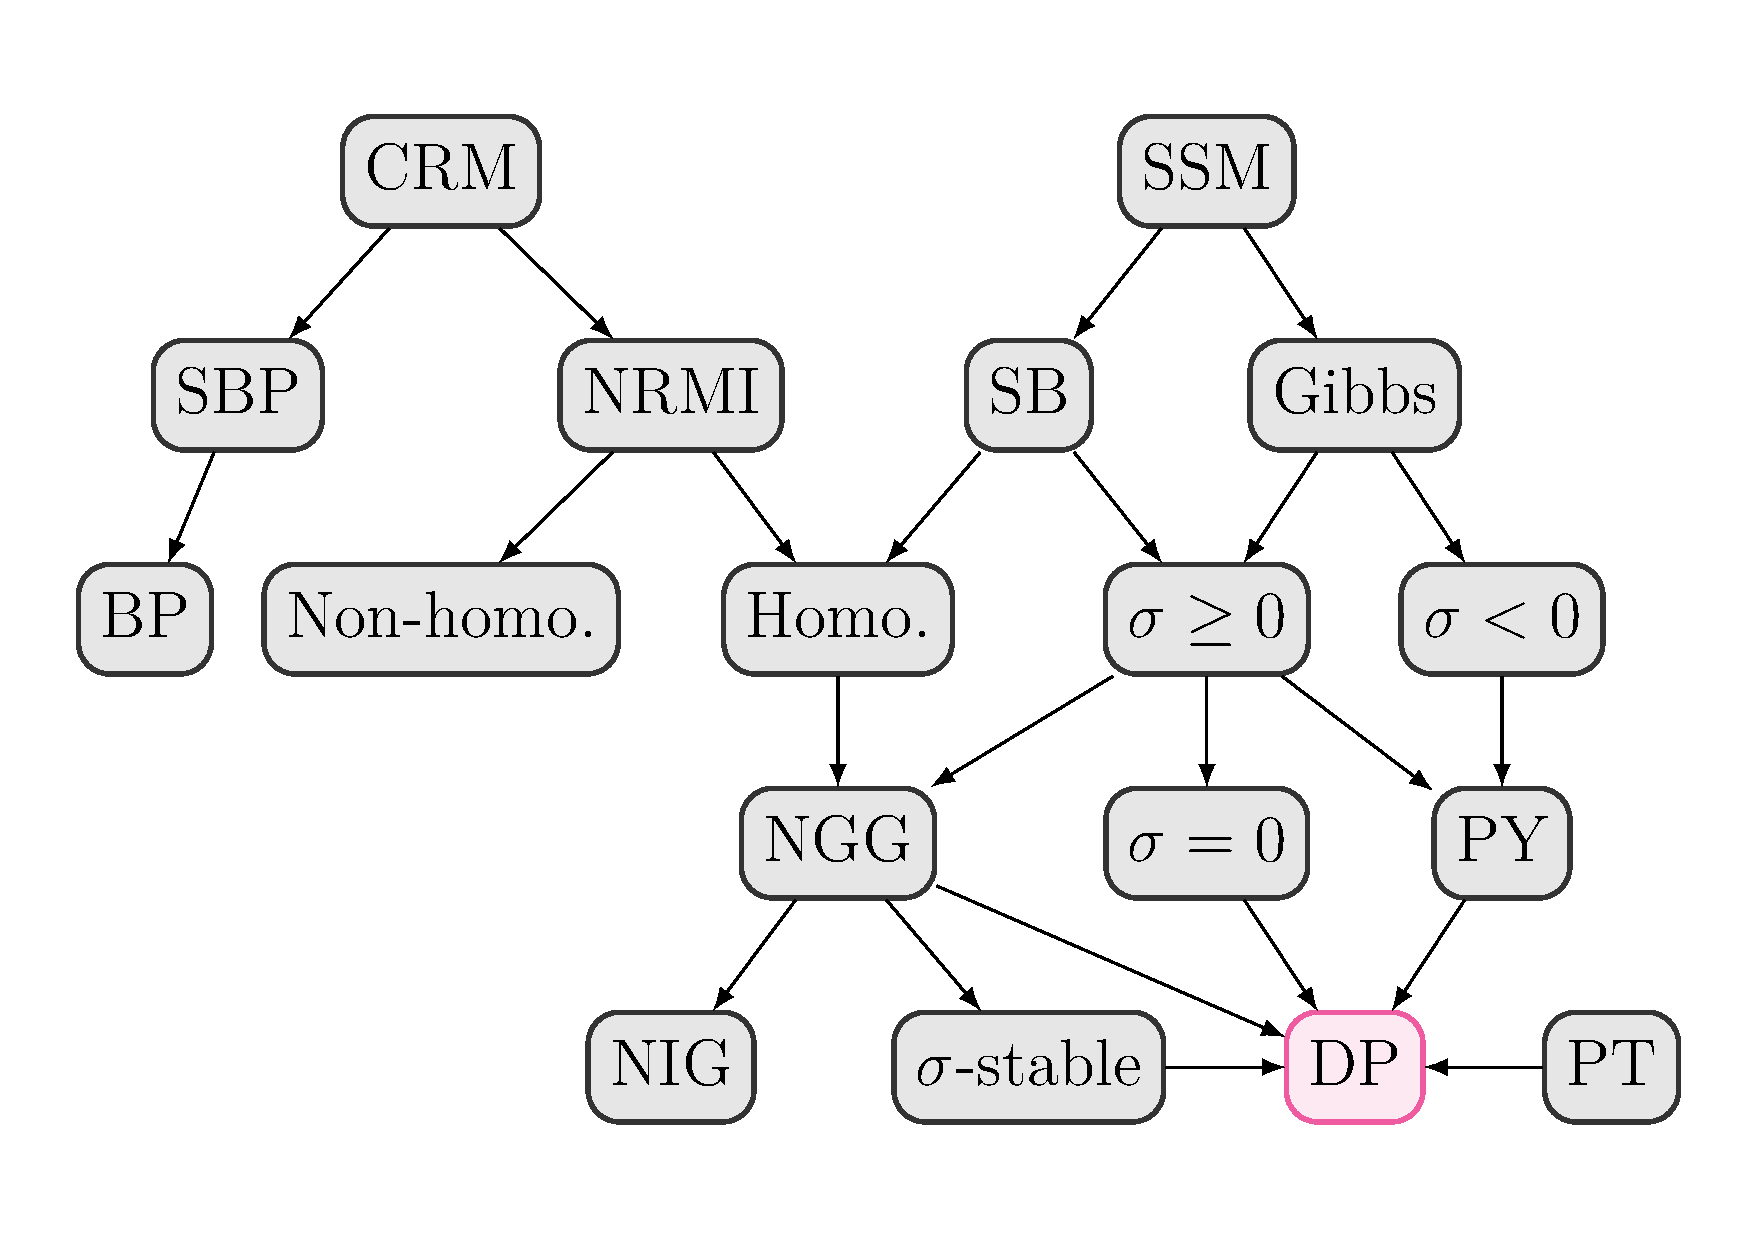
\includegraphics[width=\textwidth]{figures_julyan/introRPM/graph_model}



%------------------
% PY

\subsection{Pitman--Yor process}
	\begin{proposition}
[Pitman Sampling formula] The multiplicities $(m_1,\ldots,m_n)$ in $X_1,\ldots, X_n|P\simiid P,\ P\sim PY(\sigma, \PrecisonParam P_0)$ have distribution
\begin{equation*}
    p(m_1,\ldots,m_n)=\frac{n!}{(1+\PrecisonParam)_{(n-1)}}(\PrecisonParam +\sigma)\cdots (\PrecisonParam+(k-1)\sigma)\prod_{\ell=1}^n\frac{1}{m_\ell!}\bigg(\frac{(1-\sigma)_{(\ell-1)} }{\ell!}\bigg)^{m_\ell}
\end{equation*}
\end{proposition}


\begin{proof}
Same technique as for the Dirichlet process Ewen sampling formula.
\end{proof}




\begin{proposition}[Power law and $\sigma$-diversity]
For $\sigma >0$ we have the almost sure convergence 
$$
n^{-\sigma}K_n\rightarrow S_{\sigma, \PrecisonParam},
$$
where $ S_{\sigma, \PrecisonParam}$ is called $\sigma$-diversity of the PY, whose density is a polynomially tilted \alert{Mittag--Leffler density} (ML):
\begin{equation*}
    g_{\sigma,\PrecisonParam}(x)\propto x^{\PrecisonParam/\sigma}g_\PrecisonParam (x),
\end{equation*}
and $g_\alpha$ is ML density.
\end{proposition}

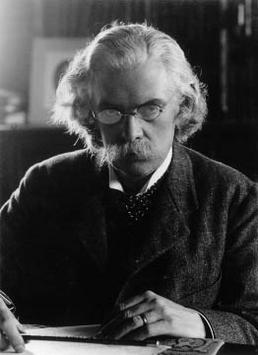
\includegraphics[width=\textwidth]{figures_julyan/trombi/Mittag-Leffler}
		\hfill\textcolor{gray}{[Image: Wikipedia]}





\begin{theorem}[Stick breaking representation for PY]
If $V_j\simind Be(1-\sigma, \PrecisonParam + j\sigma)$ and $p_1=V_1,\ p_j=V_j\prod_{l<j}(1-V_l)$ and further we have $\phi_j\simiid P_0$ then 
$$
P=\sum_{j=1}^\infty p_j \delta_{\phi_j} \sim PY(\sigma,\PrecisonParam P_0).
$$
\end{theorem}



\begin{proposition}
[Moments of PY] If $P\sim PY(\sigma, \PrecisonParam P_0)$, then for every measurable sets $A,B$ we have
\begin{enumerate}
    \item[1)] $\E [P(A)] = P_0(A),$
    \item[2)] $\E[P(A)P(B)]=(1-\sigma)/(1+\PrecisonParam)P_0(A\cap B) + (\PrecisonParam + \sigma)/(1+ \PrecisonParam)P_0(A)P_0(B),$
    \item[3)] $\Cov[P(A),P(B)] = (1-\sigma)/(1+\PrecisonParam)\big(P_0(A\cap B) -P_0(A)P_0(B)\big)$.  
\end{enumerate}
\end{proposition}


\begin{proof}
\begin{enumerate}
    \item[1)] We use the stick-breaking representation:
    \begin{equation*}
        \E P(A) =\sum_j \E p_j \E\delta_{\phi_j}=\sum_j \E(p_j) P_0(A) = P_0(A)\E (\sum_j p_j)= P_0(A).
    \end{equation*}
    \item[2)] Let $X_1, X_2|P \simiid P$, then
    \begin{equation*}
        \E(P(A)P(B)) = \mathsf{P}(X_1\in A, X_2\in B)=\mathsf{P}(X_1\in A)\mathsf{P}(X_2\in B|X_1\in A).
    \end{equation*}
    Lets investigate two terms above: from 1) we know that $\mathsf{P}(X_1\in A)=P_0(A)$. We know the predictive of PY:
    \begin{equation*}
        X_2|X_1 \sim \frac{\PrecisonParam + \sigma}{\PrecisonParam + 1}P_0+\frac{1-\sigma}{\PrecisonParam + 1}\delta_{X_1},
    \end{equation*}
    and hence
    \begin{equation*}
        \mathsf{P}(X_2\in B|X_1\in A) = \frac{\PrecisonParam + \sigma}{\PrecisonParam + 1}P_0(B) + \frac{1-\sigma}{\PrecisonParam + 1}P_{0A}(B),
    \end{equation*}
    when we used notation $P_{0A}(B)=P_0(B|A)=P_0(A\cap B)/P_0(A)$ for a conditional measure.
    \item[3)] It is straightforward combination of 1) and 2).
\end{enumerate}
\end{proof}


Unlike the DP, PY is not conjugate under incoming independent samples. However, the posterior can be explicited.

\begin{theorem}
[Posterior distribution of PY] If $P\sim PY(\sigma, \PrecisonParam P_0)$ then the posterior of $P$ based on observations $X_{1:n}|P\simiid P$ has the distribution of the random probability measure
\begin{equation*}
    (1-q_n)P_n + q_n \sum_{j=1}^{K_n}p_j^*\delta_{X_j^*},
\end{equation*}
where $X^*_{1:n}$ are the $K_n$ distinct values in $X_{1:n}$, frequencies are referred to as $n_1,\ldots,n_{K_n}$ and 
\begin{itemize}
    \item $q_n\sim Beta(n-K_n \sigma, \PrecisonParam +K_n\sigma)$,
    \item $(p_1^*, \ldots, p^*_{K_n})\sim \Dir_{K_n}(n_1-\sigma, \ldots, n_{K_n} -\sigma)$,
    \item $P_n\sim PY(\sigma, (\PrecisonParam + \sigma K_n)P_0)$.
\end{itemize}
\end{theorem} 


{Impact of the stability parameter $\sigma$}
Prior distribution of the number of clusters $k_n$ 
\begin{itemize}
\item \textcolor{red2}{$\alpha$ controls the location} (as for the DP)
\item \textcolor{red2}{$\sigma$ controls the flatness (or variability)}
\end{itemize}

Example with $n=50, \alpha=1$ and \textcolor{red2}{$\sigma=0.2,0.3,\ldots, 0.8$}

\begin{center}
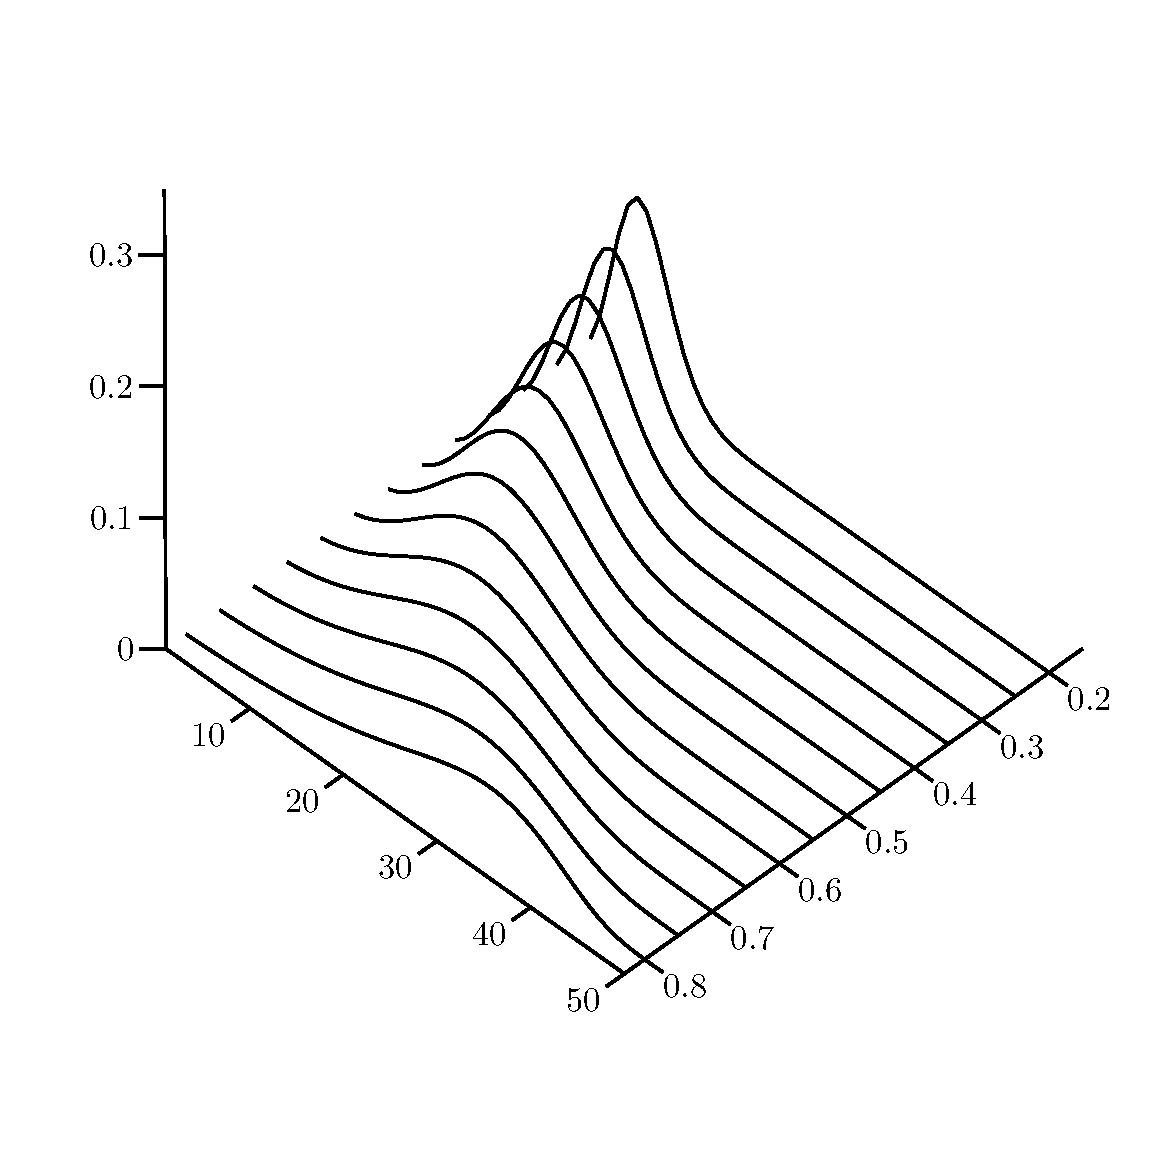
\includegraphics[width=.7\textwidth]{figures_julyan/introRPM/prior_K_n_PY.pdf}\\
	\hfill\textcolor{gray}{[Image by \citet{deblasi2015gibbs}]}
\end{center}



{Hierarchical Dirichlet process}

A nonparametric version of \textbf{Latent dirichlet allocation} \citep{blei2003latent} due to  \citet{teh2006hierarchical}\\
\begin{center}
		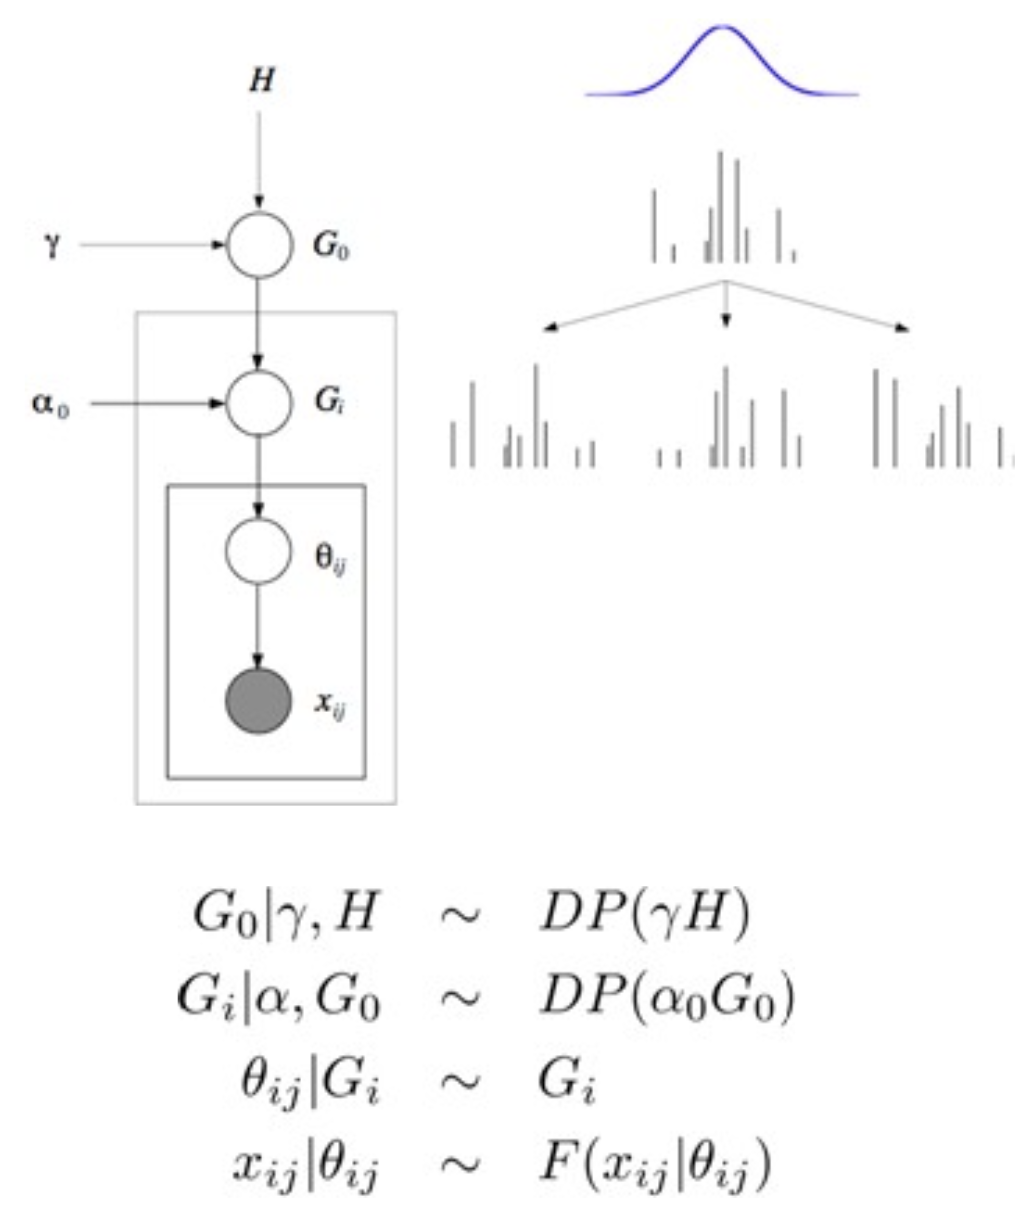
\includegraphics[width=.5\textwidth]{figures_julyan/beyond_DP/HDP}
\end{center}
\hfill\textcolor{gray}{[Image by M. Jordan]}

	
	Associated partition distr. called \alert{Chinese Restaurant Franchise}.


{Indian Buffet process}

	Feature allocation model by  \citet{ghahramani2006infinite}, where observations may share several features. 	\alert{Generative model is as follows}
	\begin{itemize}
		\item first customer samples $\text{Poisson}(\gamma)$ dishes
		\item second customer chooses every dish of first customer \textit{wp} $1/2$, plus  $\text{Poisson}(\gamma/2)$ new dishes
		\item $\ldots$
		\item $i$th step: $K$ dishes have been sampled, each by $n_1,\ldots,n_K$ customers;  $i$th customer chooses $j$th dish  \textit{wp} $n_j/i$, plus  $\text{Poisson}(\gamma/i)$ new dishes.
	\end{itemize}
	
	\alert{Log growth}: $K_n\sim \text{Poisson}(\gamma\log n)$.
	
		\begin{center}
			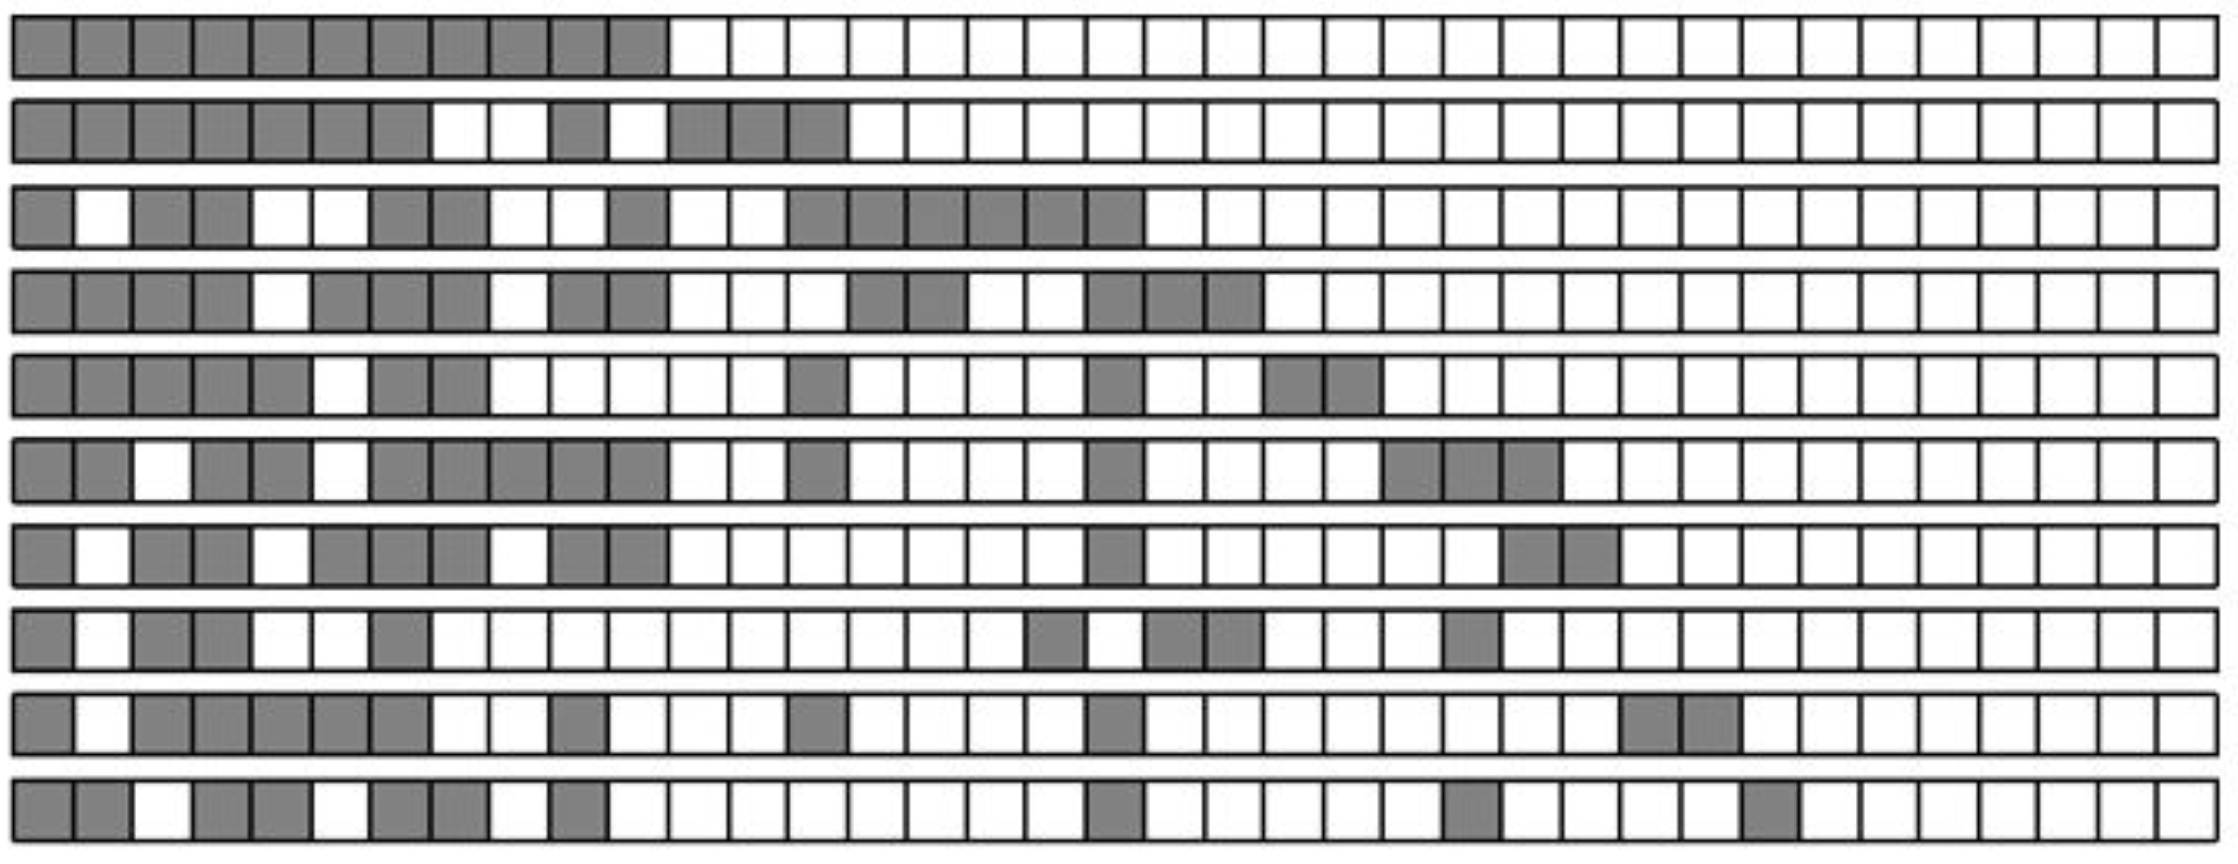
\includegraphics[width=.7\textwidth]{figures_julyan/beyond_DP/IBP_draw}
		\end{center}
		\hfill\textcolor{gray}{[Image by M. Jordan]}







